\chapter{Results}
%Figure \ref{fig:cpd_perf}, shows accuracy and detection time as a function of the
%false positive rate per second, for the OSU Hip dataset,
%for each of the SVM, Decision Tree, and Neural Net base classifiers.
%
%\begin{figure}
% \centering
% 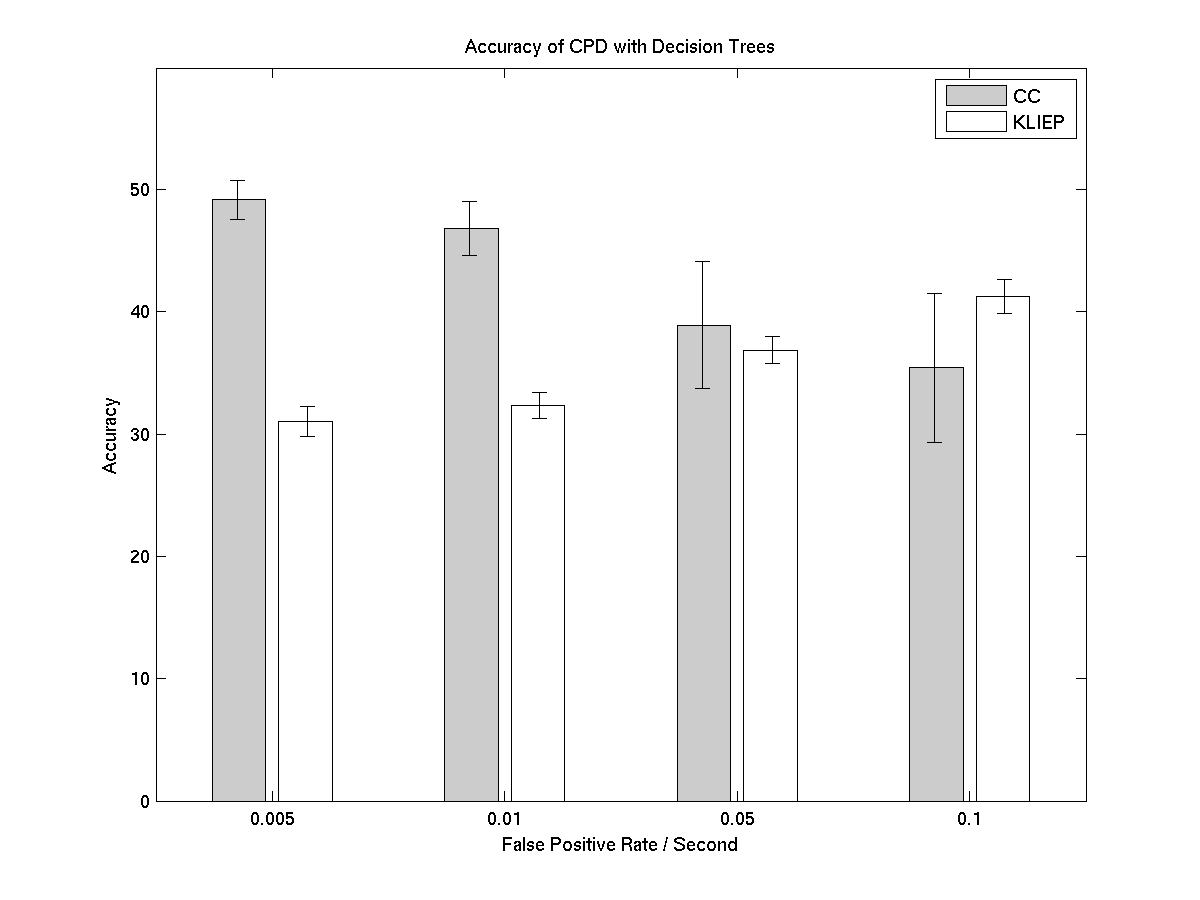
\includegraphics[scale=0.3]{osu_cpd_dt_acc.png}
% 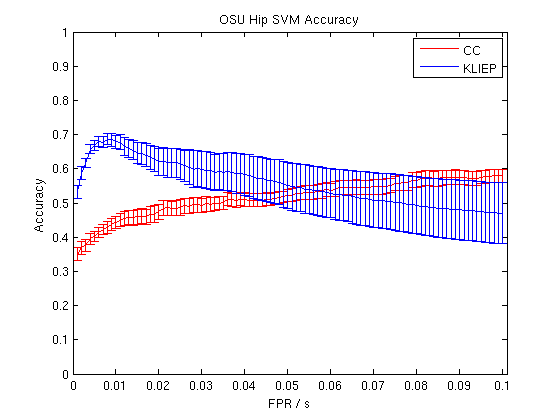
\includegraphics[scale=0.3]{osu_cpd_svm_acc.png}
% 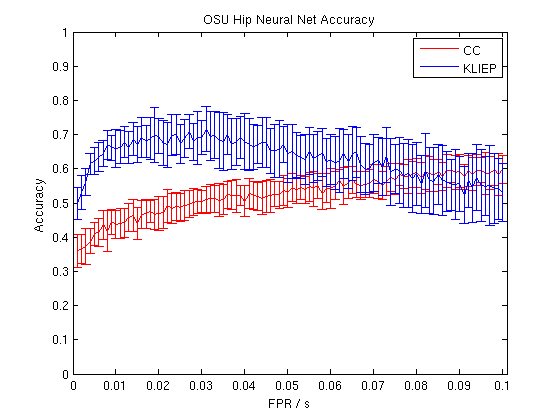
\includegraphics[scale=0.3]{osu_cpd_nnet_acc.png}
% 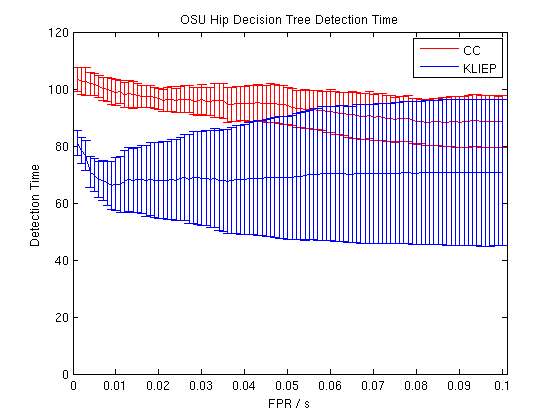
\includegraphics[scale=0.3]{osu_cpd_dt_det.png}
% 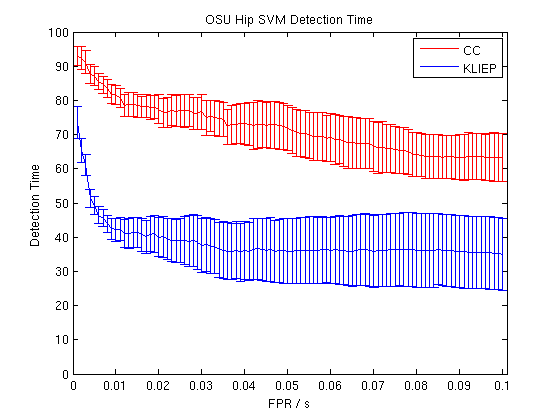
\includegraphics[scale=0.3]{osu_cpd_svm_det.png}
% 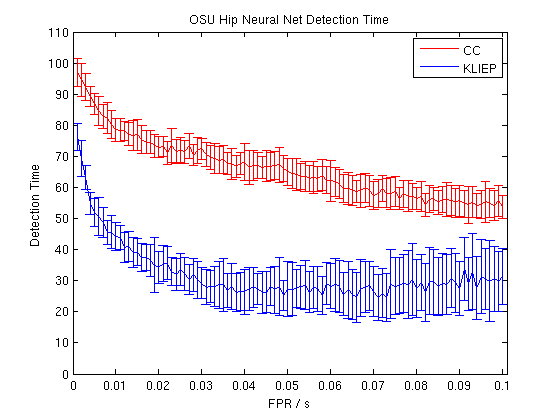
\includegraphics[scale=0.3]{osu_cpd_nnet_det.png}
% \caption{CPD-Based Classification Performance}
% \label{fig:cpd_perf}
%\end{figure}

\section{Change-Point Detection}
Results for our change-point detection experiments are given in
Figures \ref{fig:osu_cpd}-\ref{fig:lime2_cpd}.
We hypothesized that the performance of the change-point detection algorithms
would depend heavily on the threshold level for change prediction. This was
tested by varying the average number of times per second that the algorithms
falsely predicted a change. A large number of such false positive rates per
second were tested, but for the sake of brevity only a representative sample
of $\{0.005, 0.01, 0.05, 0.1\}$ are shown here.

In the OSU Hip experiments, control charts outperformed KLIEP in terms of
detection time (Figures 4.1.2, 4.1.4, 4.1.6), while the accuracy results were
mixed. It is generally expected that the accuracy curve as
a function of the false positive rate will be unimodal: very large windows
extend into multiple activities and confuse a classifier, while very small
windows do not contain enough information to be discriminative. This
unimodal behavior is shown in the control chart results, but not in the KLIEP
results (Figures 4.1.1, 4.1.3, 4.1.5). Follow-up experiments showed that the peak
in KLIEP accuracy performance occurred between false positive rates of $0.2$ and
$0.3$ for each of the three classifiers.

Further investigation indicated that across the OSU Hip dataset the KLIEP algorithm
was unable to detect many different activity changes without a very low score
threshold value (and consequently very high false positive rates).
Some qualitative plotting of the OSU Hip data showed
that most of its activities have accelerometer amplitude values that strongly
resemble draws from a multivariate normal distribution. Since control charts
assume that the data is drawn from a distribution that is a member of that
family, it is logical that control charts would outperform algorithms with
different modeling assumptions on OSU Hip.

In the LiME experiments, KLIEP outperformed control charts in terms of
accuracy across the board, and control charts outperformed KLIEP in terms of
detection time across the board. (TODO: Need to interpret this, but not sure
how.)

Finally, in a few cases (Figures 4.1.2, 4.1.6, 4.2.6) the detection time did
not decrease as the false positive rate increased. On the face of it this would seem
to be a non-sequitur, but this only happened in cases when accuracy also decreased
(Figures 4.1.1, 4.1.5, 4.2.5).
Smaller window sizes tend to be correlated with decreased detection times, but
it is possible that predicting on smaller windows, if they happen to be less discriminative,
can actually increase the time required for the classifier to start correctly
predicting the ground-truth activity. Additionally, the given increases in detection
time were small and near standard error.

%\setlength{\abovecaptionskip}{-5pt}

\begin{table}[h]
\captionsetup{font=scriptsize}
\begin{center}
\tiny{
\begin{tabular}{ cc|c|c|c|c|c|c|c|c|c|c|c|c| }
\cline{3-14}
& & \multicolumn{4}{ c| }{DT} & \multicolumn{4}{ c| }{SVM} & \multicolumn{4}{ c| }{NNET}\\ \cline{3-14}
& & 0.005 & 0.01 & 0.05 & 0.1 & 0.005 & 0.01 & 0.05 & 0.1 & 0.005 & 0.01 & 0.05 & 0.1\\ \cline{1-14}
\multicolumn{1}{ |c| }{\multirow{2}{*}{OSU Hip}} &
\multicolumn{1}{ |c| }{CC} & 49.2 & 46.8 & 38.9 & 35.4 & 66.8 & \textbf{67.9} & 55.2 & 47.0 & 62.3 & 65.9 & 64.5 & 53.1\\ \cline{2-14}
\multicolumn{1}{ |c }{} &
\multicolumn{1}{ |c| }{KLIEP} & 31.0 & 32.3 & 36.9 & 41.3 & 40.3 & 44.3 & 52.1 & 58.0 & 41.0 & 43.8 & 53.0 & \textbf{59.9}\\ \cline{1-14}
\multicolumn{1}{ |c| }{\multirow{2}{*}{LiME Day 1}} &
\multicolumn{1}{ |c| }{CC} & 47.5 & 48.2 & 43.0 & 41.9 & \textbf{57.7} & 57.3 & 52.0 & 51.4 & 19.1 & 21.0 & 17.4 & 16.8\\ \cline{2-14}
\multicolumn{1}{ |c }{} &
\multicolumn{1}{ |c| }{KLIEP} & 58.8 & 57.6 & 53.8 & 52.3 & \textbf{68.7} & 66.7 & 61.9 & 59.2 & 23.6 & 20.8 & 22.9 & 19.0\\ \cline{1-14}
\multicolumn{1}{ |c| }{\multirow{2}{*}{LiME Day 2}} &
\multicolumn{1}{ |c| }{CC} & \textbf{54.0} & 53.6 & 50.3 & 50.2 & 53.3 & 52.5 & 49.5 & 45.9 & 21.6 & 19.7 & 17.3 & 15.4\\ \cline{2-14}
\multicolumn{1}{ |c }{} &
\multicolumn{1}{ |c| }{KLIEP} & 63.4 & 61.5 & 59.0 & 58.6 & \textbf{65.5} & 63.2 & 58.1 & 55.8 & 25.6 & 20.0 & 20.1 & 19.6\\ \cline{1-14}
\end{tabular}
}
\end{center}
\caption{CPD Accuracy}
\label{tbl:cpd_acc}
\end{table}

\begin{table}[h]
\captionsetup{font=scriptsize}
\begin{center}
\tiny{
\begin{tabular}{ c|c|c|c|c|c|c| }
\cline{2-7}
 & \multicolumn{2}{ c| }{DT} & \multicolumn{2}{ c| }{SVM} & \multicolumn{2}{ c| }{NNET}\\ \cline{2-7}
 & 20 & 10 & 20 & 10 & 20 & 10\\ \cline{1-7}
\multicolumn{1}{ |c| }{OSU Hip}
 & 89.5 & 88.1 & \textbf{94.9} & 94.4 & 71.2 & 62.2\\ \cline{1-7}
\multicolumn{1}{ |c| }{LiME Day 1}
 & 84.3 & 83.3 & 78.3 & \textbf{84.8} & 69.6 & 51.7\\ \cline{1-7}
\multicolumn{1}{ |c| }{LiME Day 2}
 & \textbf{87.5} & 85.6 & 79.4 & 86.4 & 57.7 & 78.4\\ \cline{1-7}
\end{tabular}
}
\end{center}
\caption{HMM Accuracy}
\label{tbl:hmm_acc}
\end{table}

\begin{table}[h]
\captionsetup{font=scriptsize}
\begin{center}
\tiny{
\begin{tabular}{ cc|c|c|c|c|c|c|c|c|c|c|c|c| }
\cline{3-14}
& & \multicolumn{4}{ c| }{DT} & \multicolumn{4}{ c| }{SVM} & \multicolumn{4}{ c| }{NNET}\\ \cline{3-14}
& & 0.005 & 0.01 & 0.05 & 0.1 & 0.005 & 0.01 & 0.05 & 0.1 & 0.005 & 0.01 & 0.05 & 0.1\\ \cline{1-14}
\multicolumn{1}{ |c| }{\multirow{2}{*}{OSU Hip}} &
\multicolumn{1}{ |c| }{CC} & 69.7 & 66.5 & 68.8 & 70.7 & 49.3 & 42.2 & 35.9 & 35.0 & 52.0 & 44.2 & \textbf{27.2} & 31.3\\ \cline{2-14}
\multicolumn{1}{ |c }{} &
\multicolumn{1}{ |c| }{KLIEP} & 101.6 & 98.9 & 94.0 & 88.5 & 87.1 & 81.6 & 71.8 & 63.3 & 86.9 & 78.6 & 65.1 & \textbf{53.8}\\ \cline{1-14}
\multicolumn{1}{ |c| }{\multirow{2}{*}{LiME Day 1}} &
\multicolumn{1}{ |c| }{CC} & 107.2 & 76.9 & 56.0 & 51.3 & 79.1 & 55.5 & 36.6 & \textbf{32.8} & 168.8 & 111.1 & 78.2 & 76.8\\ \cline{2-14}
\multicolumn{1}{ |c }{} &
\multicolumn{1}{ |c| }{KLIEP} & 146.1 & 116.0 & 59.7 & 50.9 & 113.5 & 88.7 & 43.8 & \textbf{36.0} & 237.9 & 191.4 & 92.5 & 82.3\\ \cline{1-14}
\multicolumn{1}{ |c| }{\multirow{2}{*}{LiME Day 2}} &
\multicolumn{1}{ |c| }{CC} & 103.7 & 80.4 & 59.8 & 54.3 & 101.8 & 72.2 & 52.1 & \textbf{48.8} & 161.5 & 130.2 & 78.6 & 72.0\\ \cline{2-14}
\multicolumn{1}{ |c }{} &
\multicolumn{1}{ |c| }{KLIEP} & 136.0 & 121.3 & 63.2 & 54.8 & 127.3 & 112.3 & 58.4 & \textbf{50.4} & 242.6 & 216.6 & 109.2 & 88.3\\ \cline{1-14}
\end{tabular}
}
\end{center}
\caption{CPD Detection Time}
\label{tbl:cpd_det}
\end{table}

\begin{table}[h]
\captionsetup{font=scriptsize}
\begin{center}
\tiny{
\begin{tabular}{ c|c|c|c|c|c|c| }
\cline{2-7}
 & \multicolumn{2}{ c| }{DT} & \multicolumn{2}{ c| }{SVM} & \multicolumn{2}{ c| }{NNET}\\ \cline{2-7}
 & 20 & 10 & 20 & 10 & 20 & 10\\ \cline{1-7}
\multicolumn{1}{ |c| }{OSU Hip}
 & 9.8 & 9.8 & 4.5 & \textbf{4.2} & 31.4 & 40.1\\ \cline{1-7}
\multicolumn{1}{ |c| }{LiME Day 1}
 & 57.1 & 32.2 & 103.5 & \textbf{25.0} & 177.7 & 146.3\\ \cline{1-7}
\multicolumn{1}{ |c| }{LiME Day 2}
 & 47.8 & \textbf{31.7} & 101.2 & 31.8 & 255.5 & 53.7\\ \cline{1-7}
\end{tabular}
}
\end{center}
\caption{HMM Detection Time}
\label{tbl:hmm_det}
\end{table}

\setlength{\abovecaptionskip}{10pt}


\begin{figure}[H]
 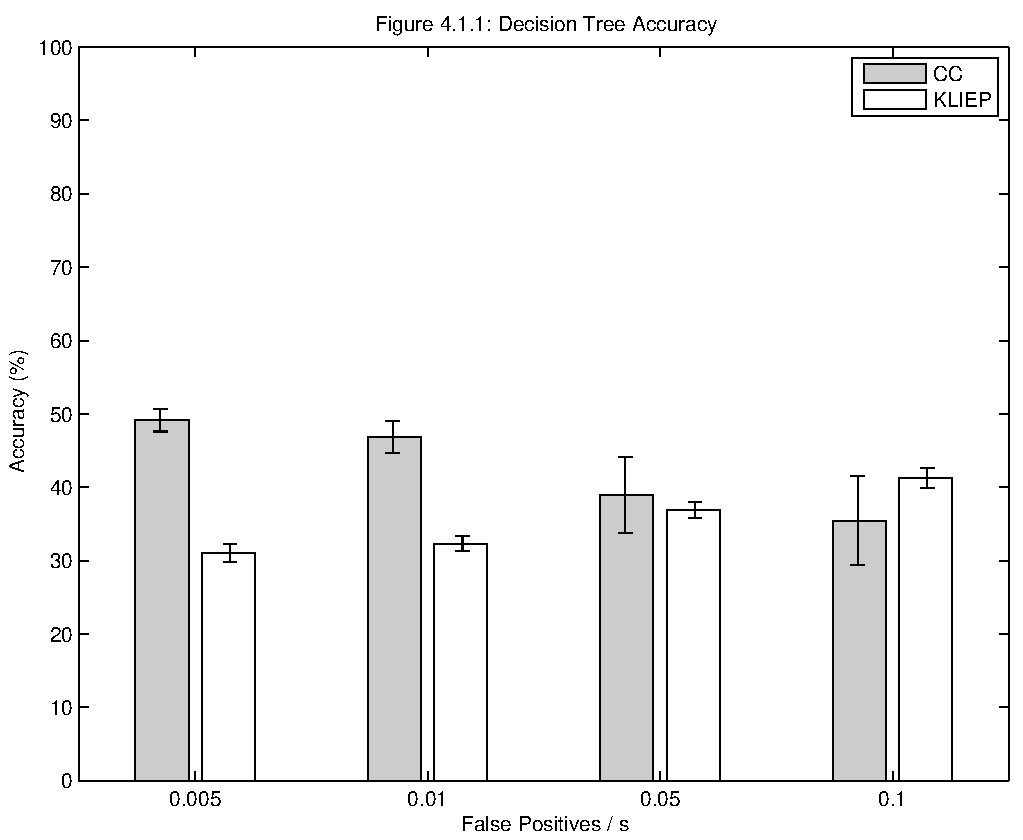
\includegraphics[scale=0.4]{osu_cpd_dt_acc.pdf} \hspace{1em}\vspace{1em}
 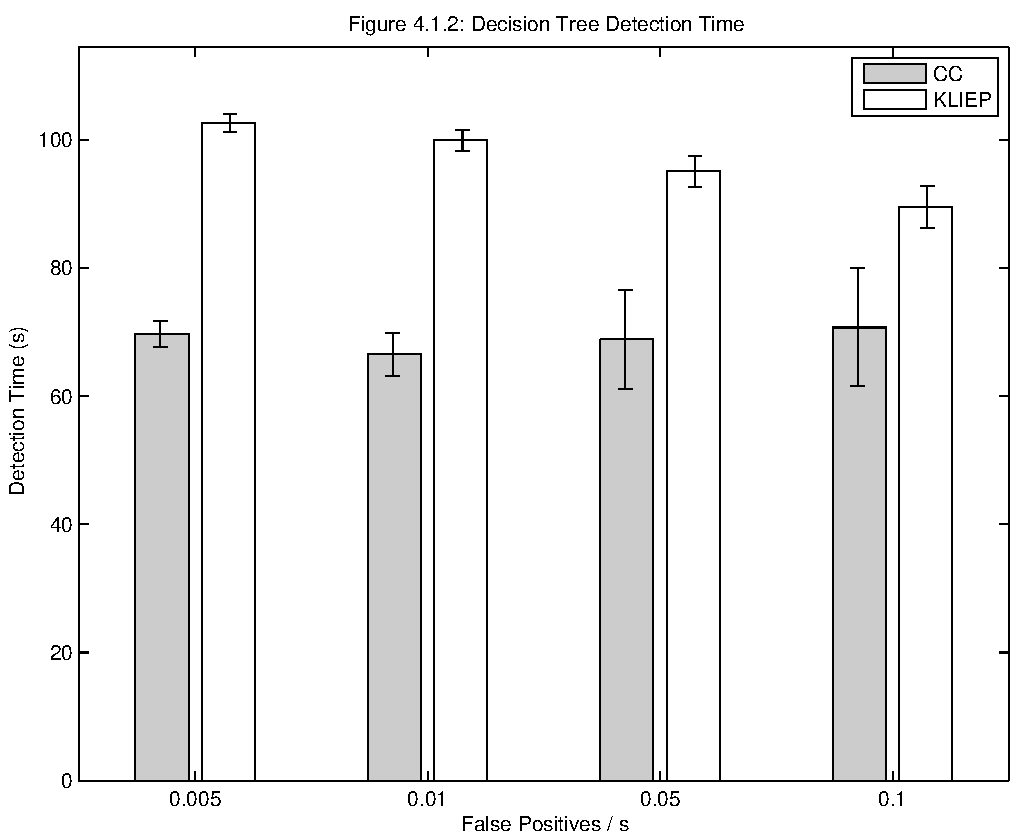
\includegraphics[scale=0.4]{osu_cpd_dt_det.pdf}
 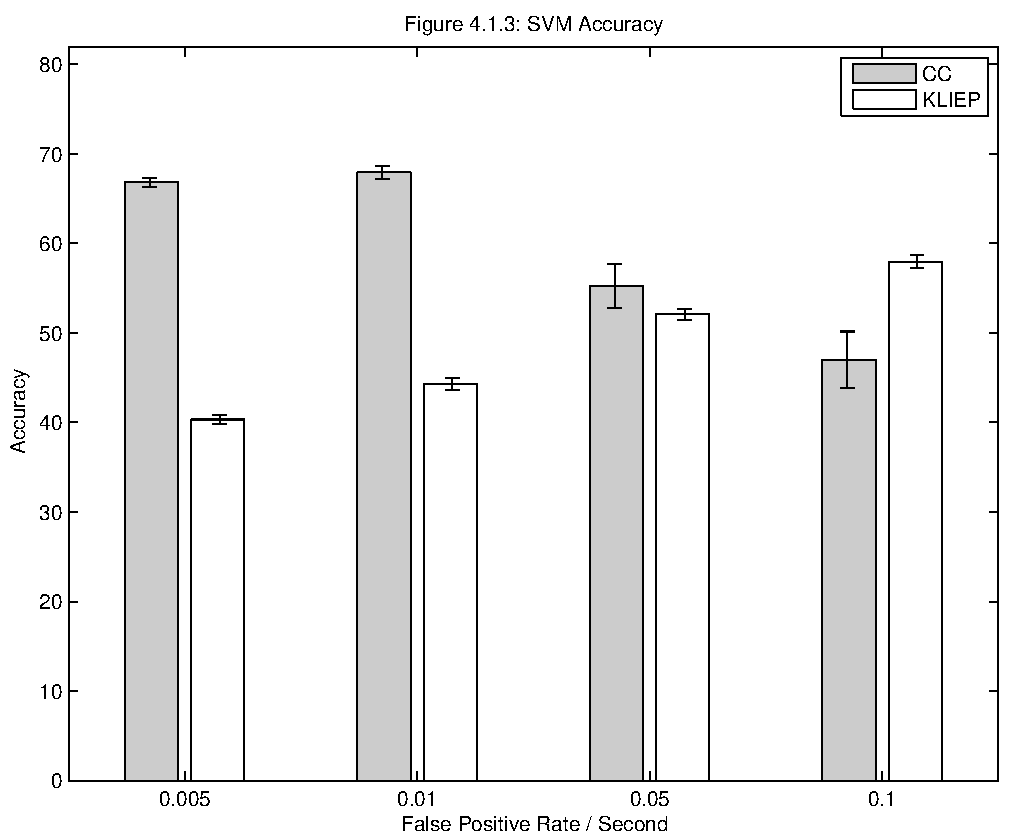
\includegraphics[scale=0.4]{osu_cpd_svm_acc.pdf} \hspace{1em}\vspace{1em}
 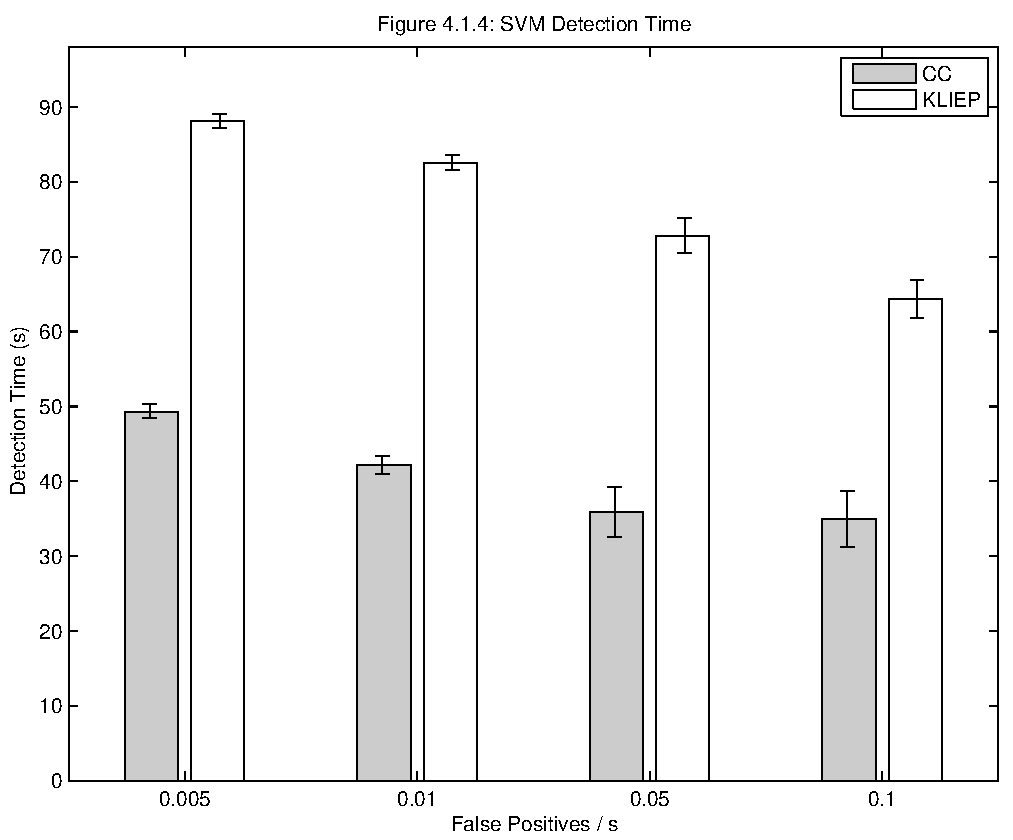
\includegraphics[scale=0.4]{osu_cpd_svm_det.pdf}
 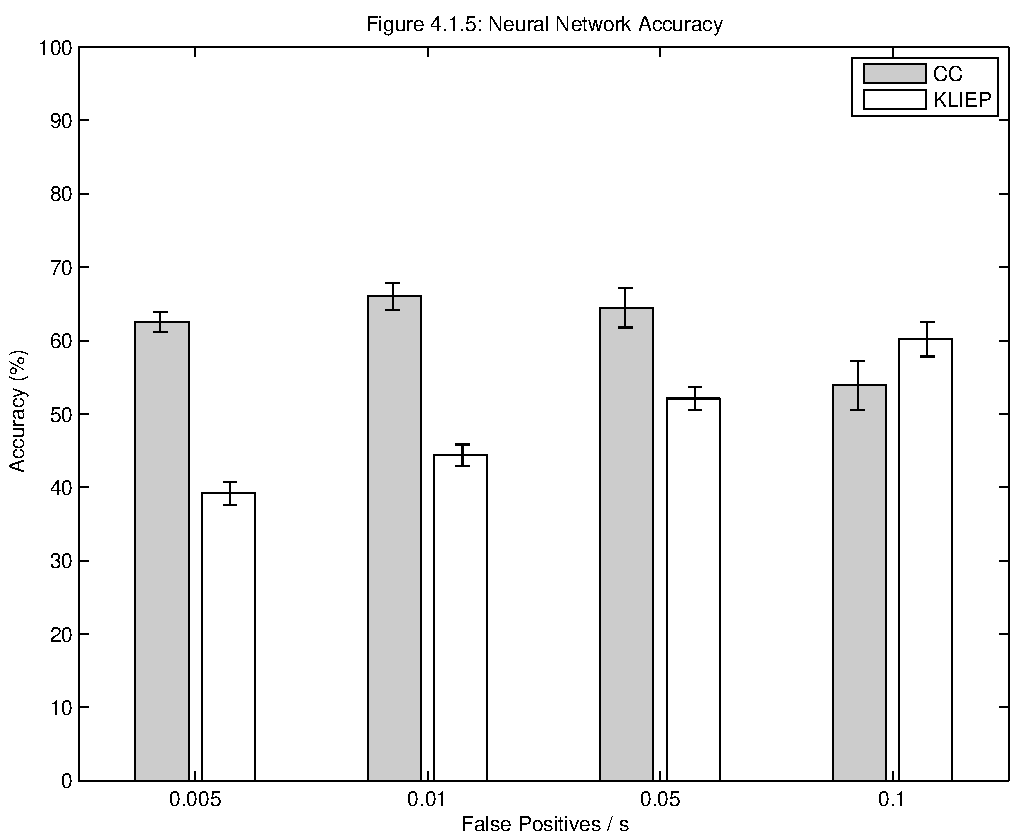
\includegraphics[scale=0.4]{osu_cpd_nnet_acc.pdf} \hspace{2em}
 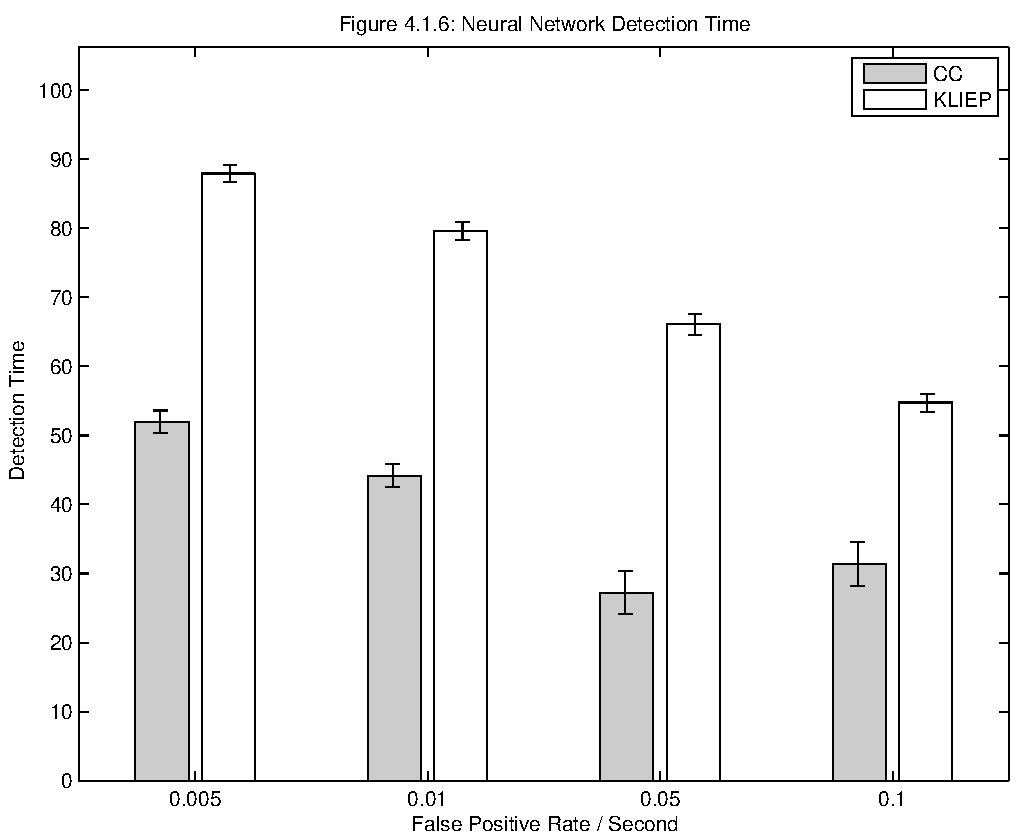
\includegraphics[scale=0.4]{osu_cpd_nnet_det.pdf}
 \caption{OSU Hip Results. Graphs are organized into rows by base classifier,
  and columns by evaluation metric. Change-point detection result were averaged over
  30 splits into training, testing, and validation datasets,
  along with bars showing one standard error.}
 \label{fig:osu_cpd}
\end{figure}

\begin{figure}[H]
 \centering
 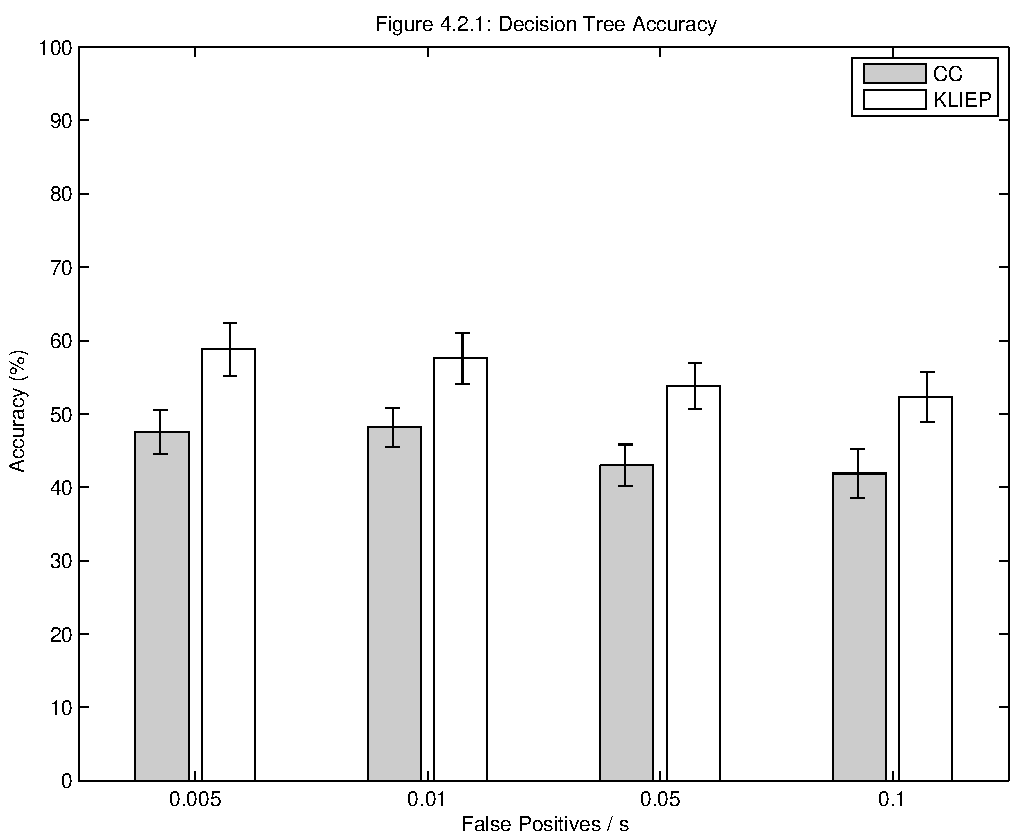
\includegraphics[scale=0.4]{lime1_cpd_dt_acc.pdf} \hspace{1em}\vspace{1em}
 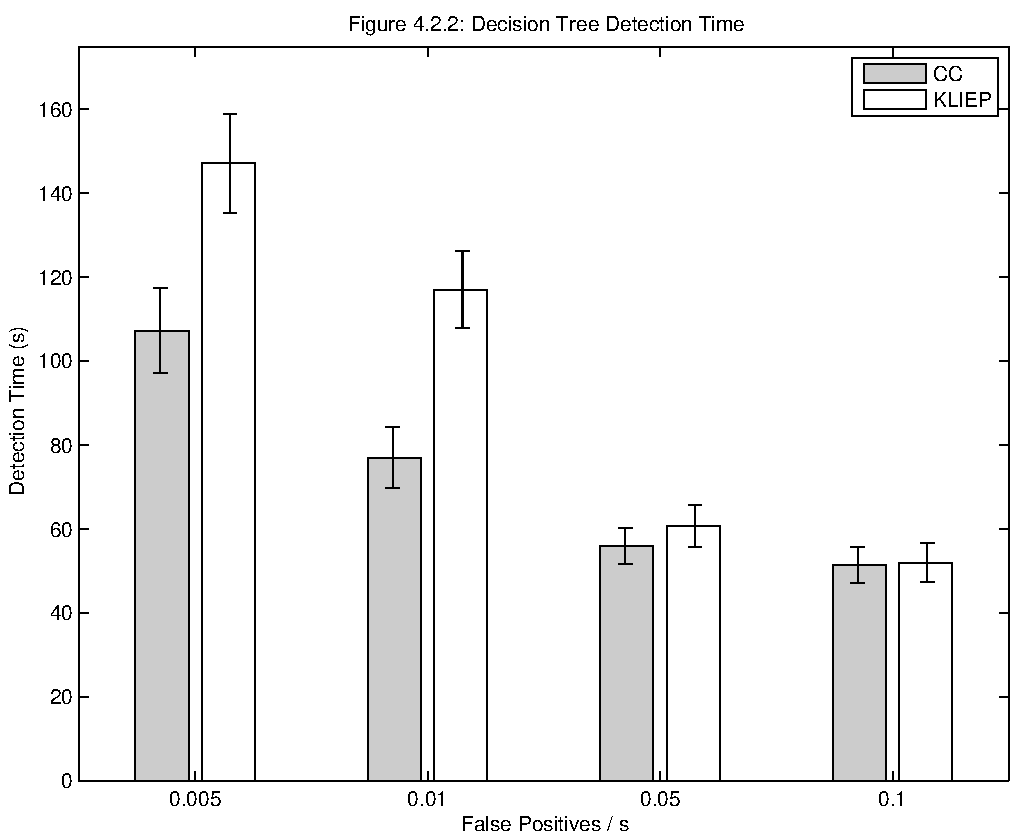
\includegraphics[scale=0.4]{lime1_cpd_dt_det.pdf}
 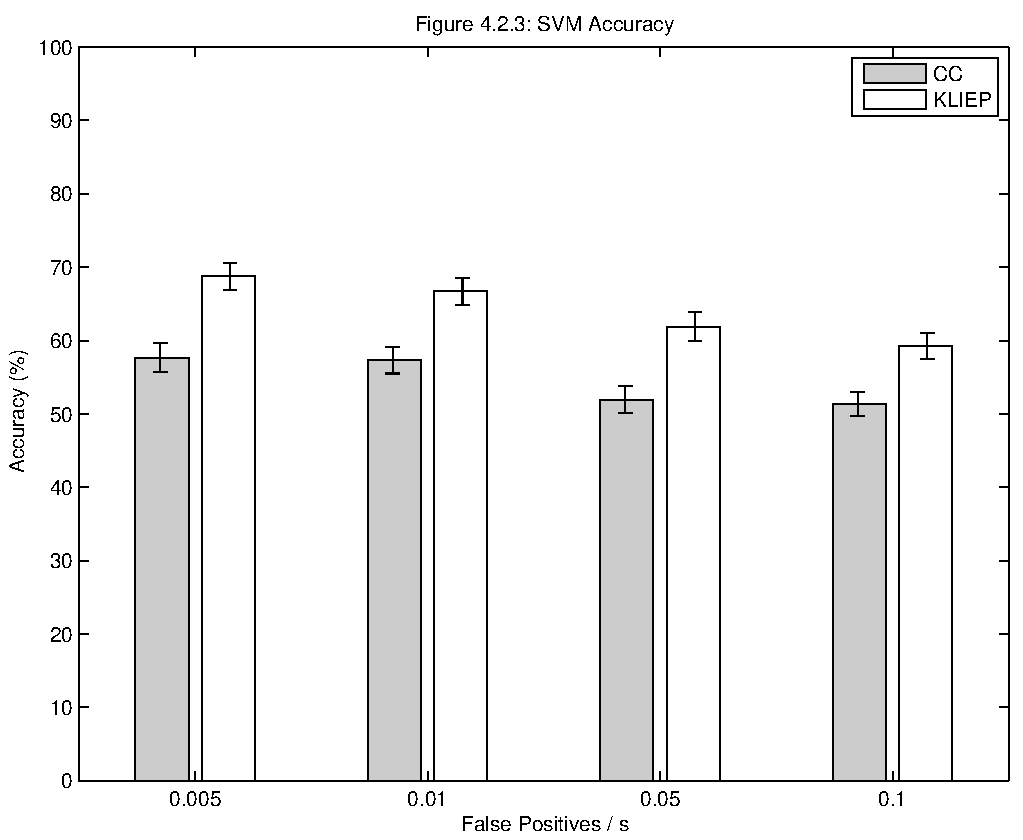
\includegraphics[scale=0.4]{lime1_cpd_svm_acc.pdf} \hspace{1em}\vspace{1em}
 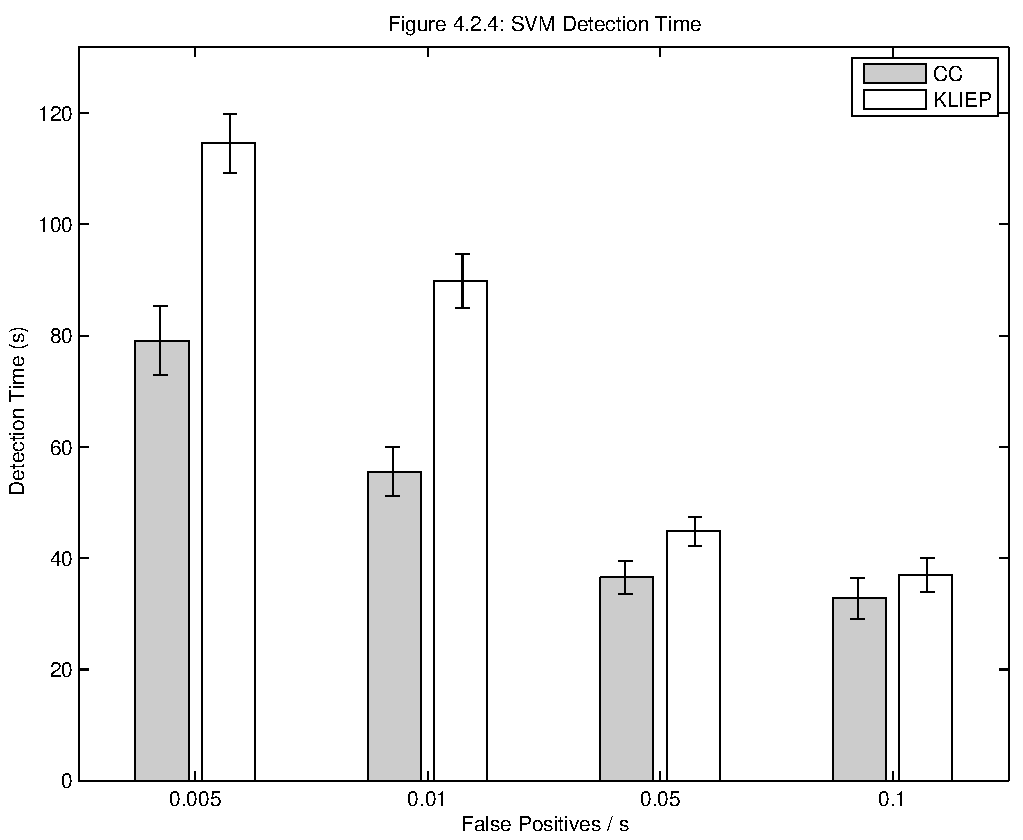
\includegraphics[scale=0.4]{lime1_cpd_svm_det.pdf}
 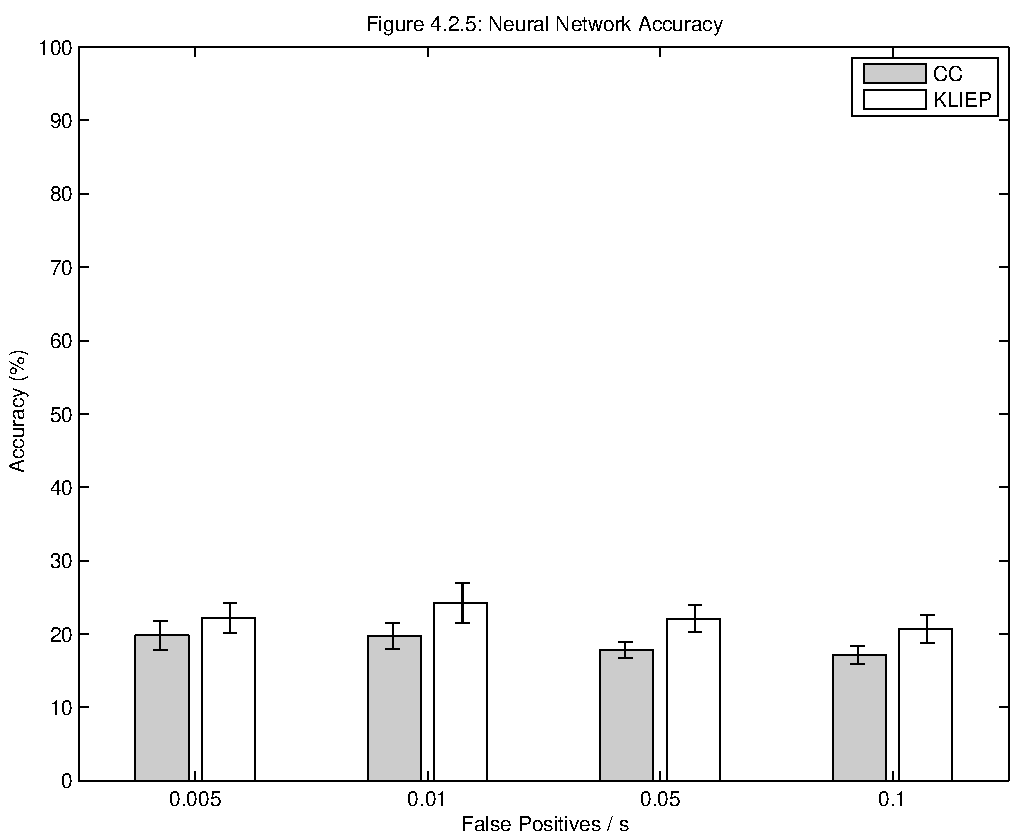
\includegraphics[scale=0.4]{lime1_cpd_nnet_acc.pdf} \hspace{1em}
 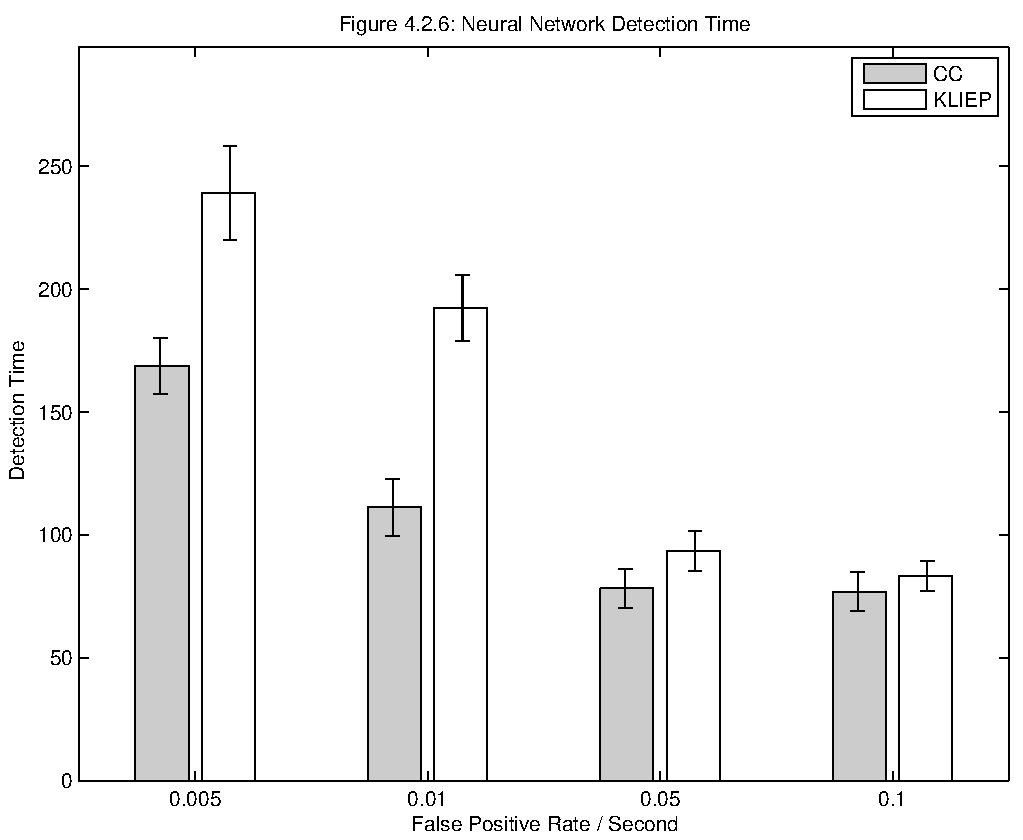
\includegraphics[scale=0.4]{lime1_cpd_nnet_det.pdf}
 \caption{LiME Day 1 Results}
 \label{fig:lime1_cpd}
\end{figure}

\begin{figure}[H]
 \centering
 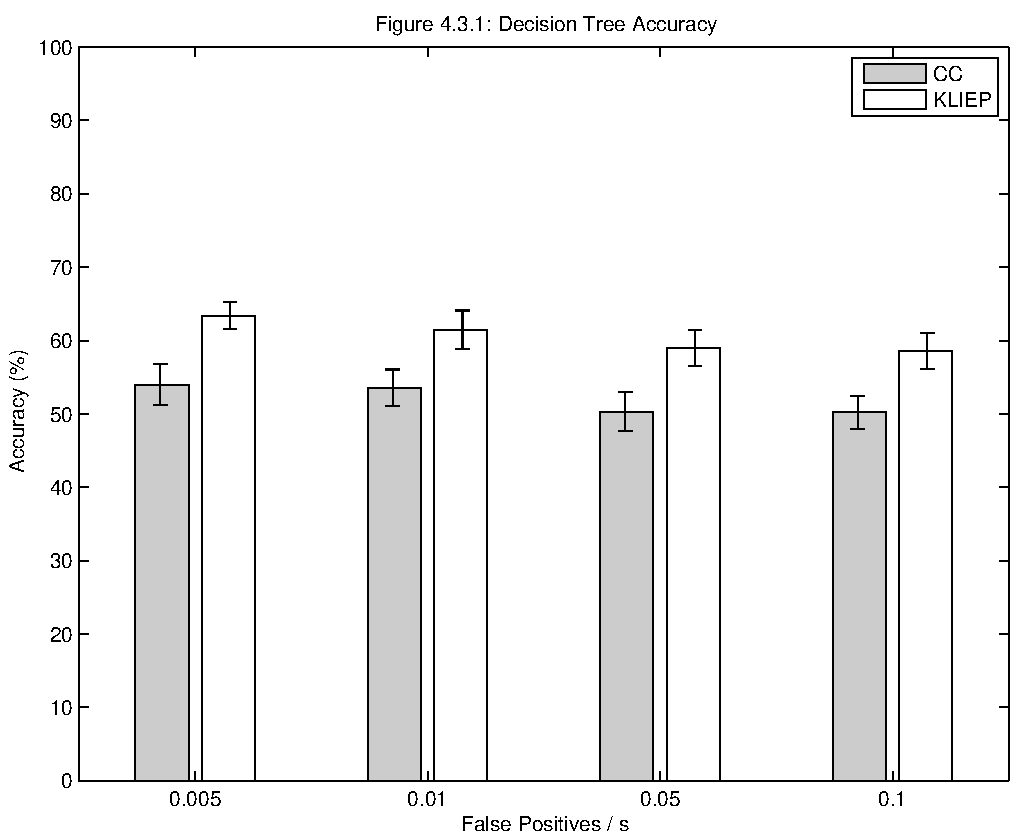
\includegraphics[scale=0.4]{lime2_cpd_dt_acc.pdf} \hspace{1em}\vspace{1em}
 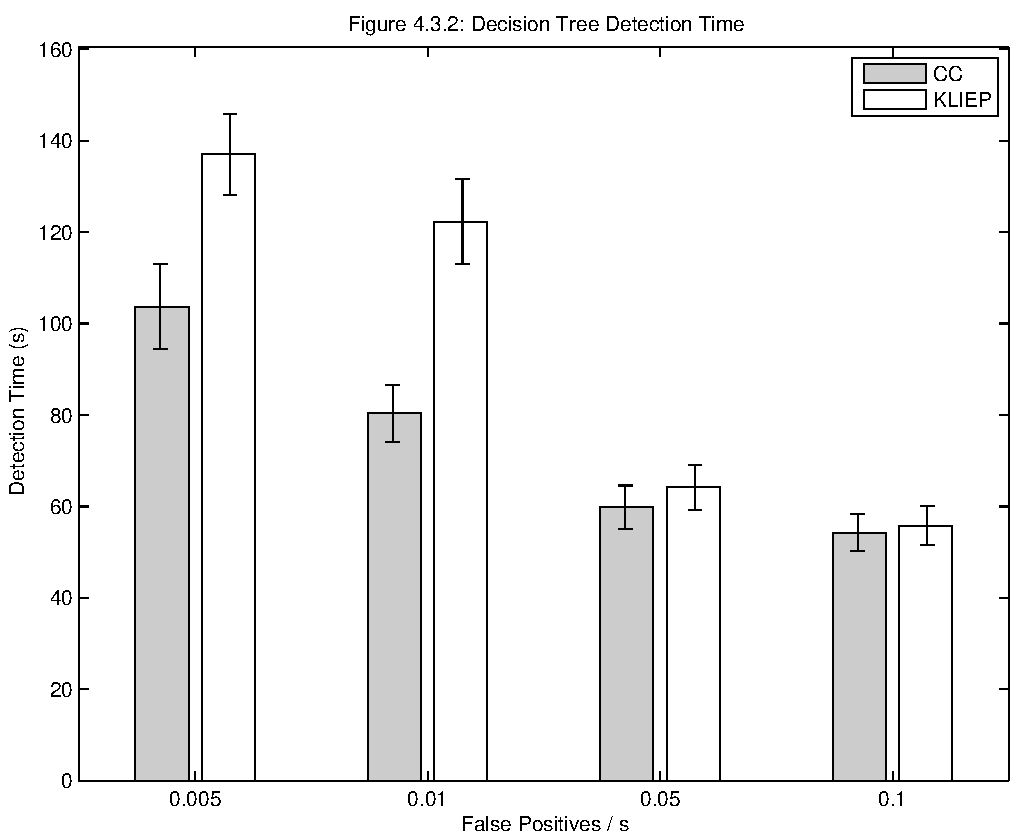
\includegraphics[scale=0.4]{lime2_cpd_dt_det.pdf}
 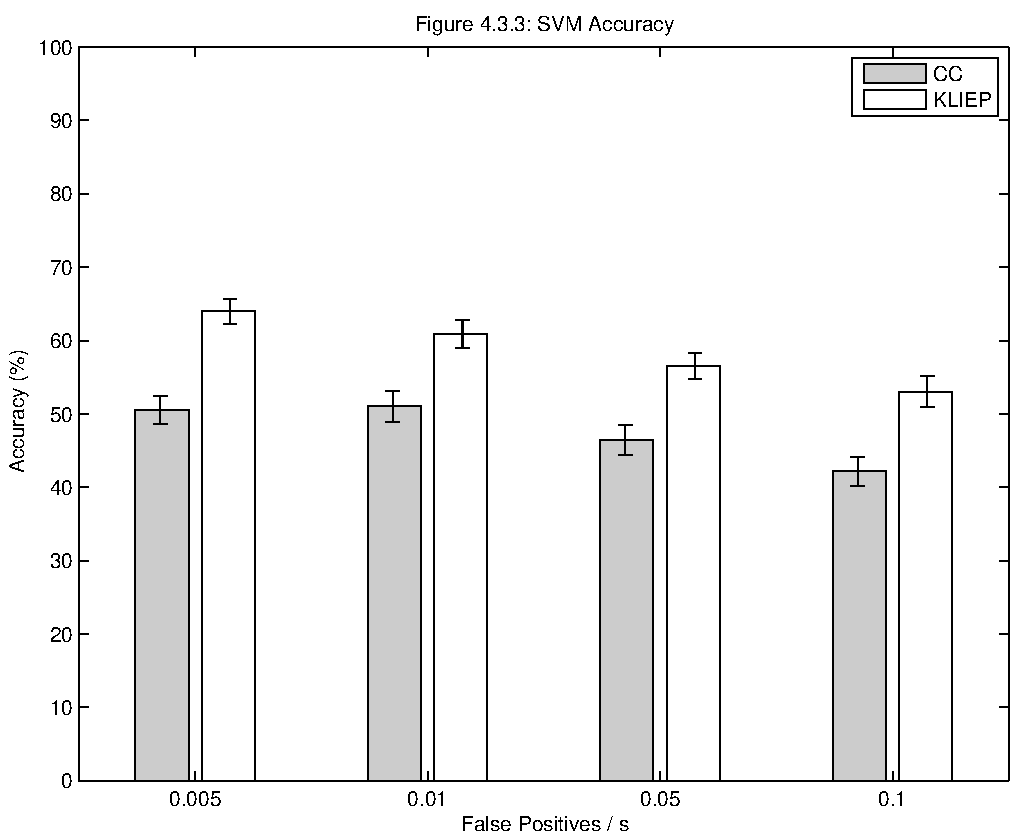
\includegraphics[scale=0.4]{lime2_cpd_svm_acc.pdf} \hspace{1em}\vspace{1em}
 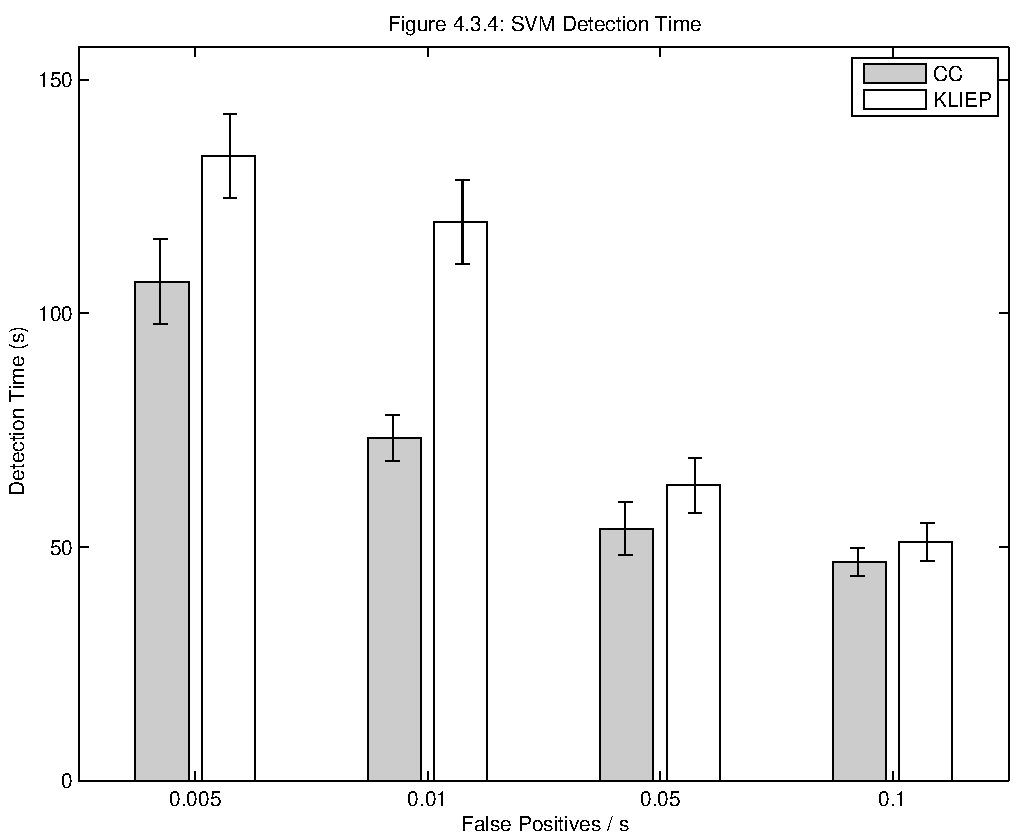
\includegraphics[scale=0.4]{lime2_cpd_svm_det.pdf}
 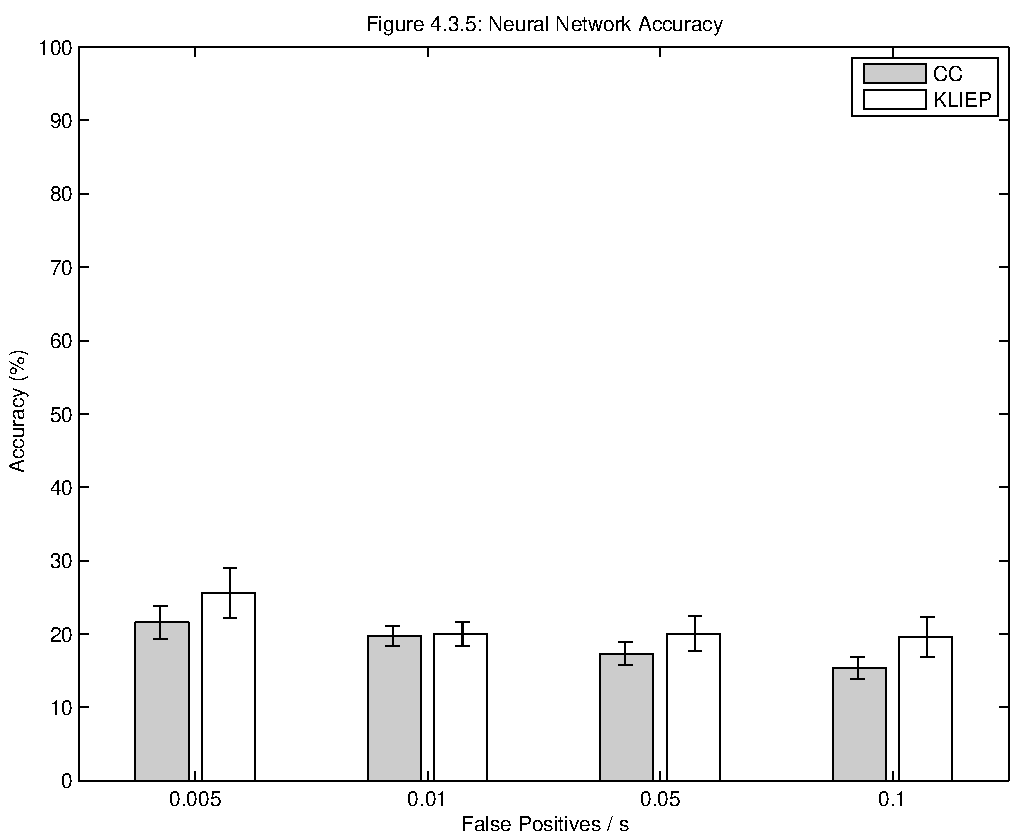
\includegraphics[scale=0.4]{lime2_cpd_nnet_acc.pdf} \hspace{1em}
 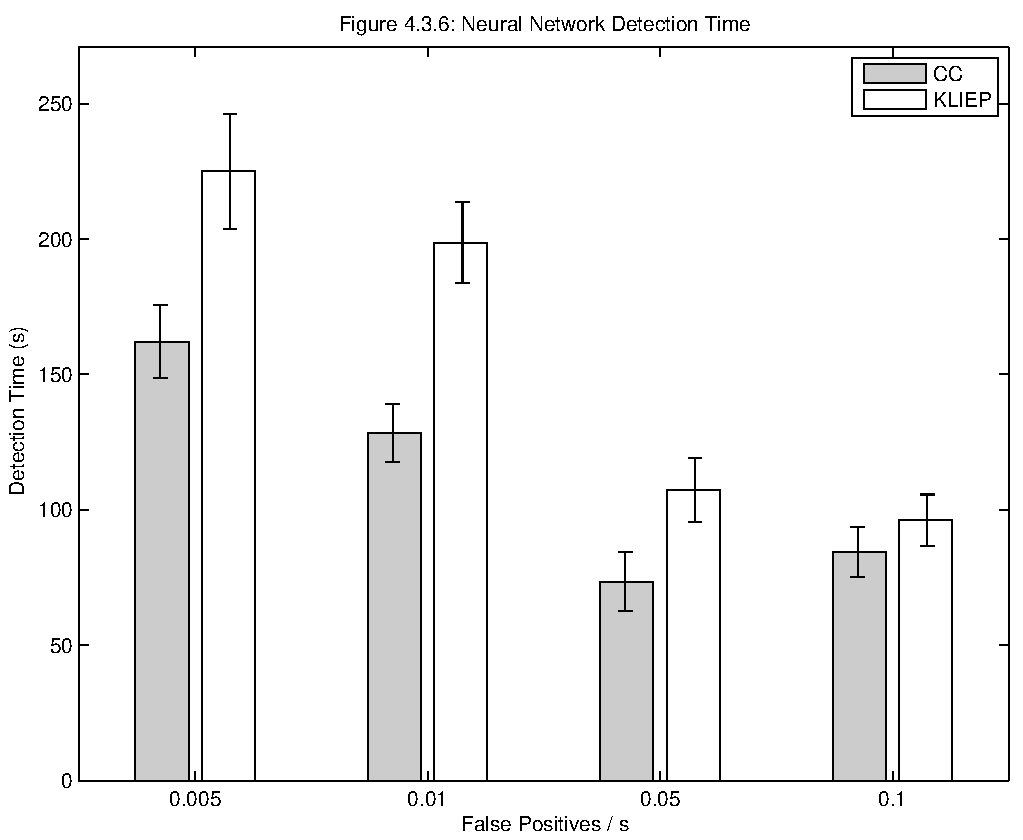
\includegraphics[scale=0.4]{lime2_cpd_nnet_det.pdf}
 \caption{LiME Day 2 Results}
 \label{fig:lime2_cpd}
\end{figure}


\section{HMM}

Results for our HMM experiments are given in
Figures \ref{fig:osu_hmm}-\ref{fig:lime2_hmm}. Each HMM experiment was
performed by splitting time series into windows of fixed length for
featurization, and results for windows of length $\{10, 12, 14, 16, 18, 20\}$
seconds are shown.

For both the SVM and decision tree classifiers, accuracy and detection time
was strong across all three datasets, and also stable with respect to window
size. Further experiments on the OSU Hip dataset showed that the HMM when
paired with these classifiers
tends to be stable with window sizes that are greater than a few seconds,
which seems to be the amount of time required to be informative. Neural networks
performed somewhat more poorly and erratically across the board.

\begin{figure}[H]
 \centering
 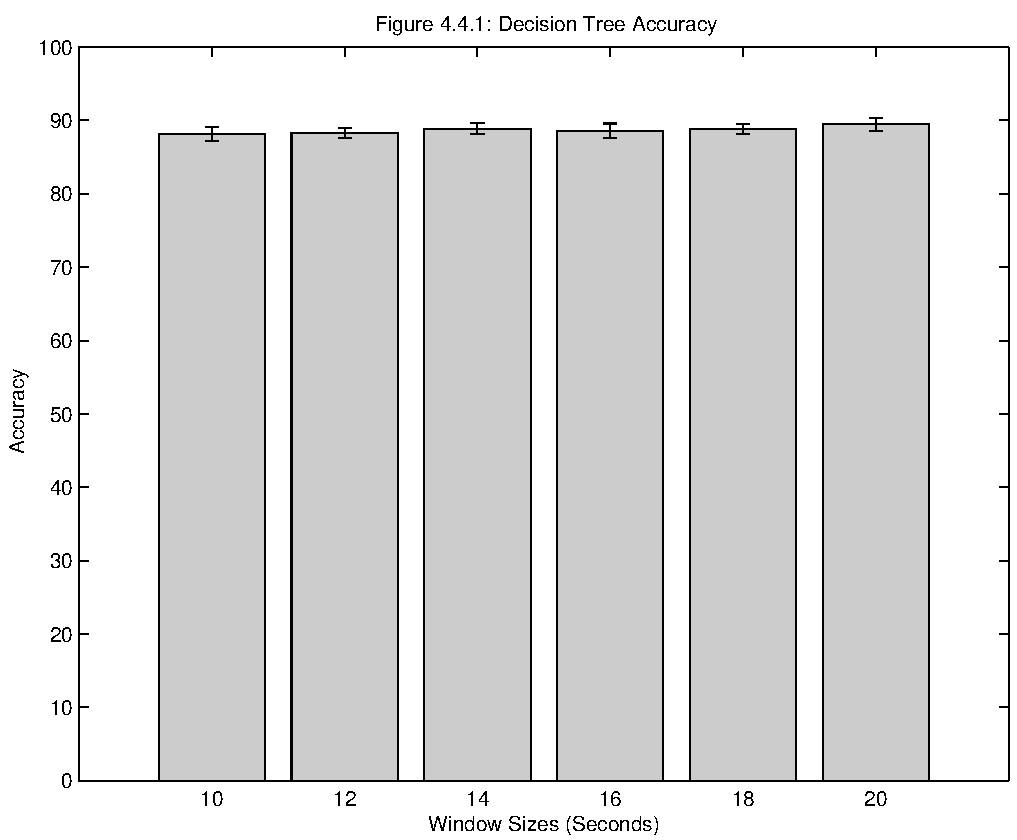
\includegraphics[scale=0.4]{osu_hmm_dt_acc.pdf} \hspace{1em}\vspace{1em}
 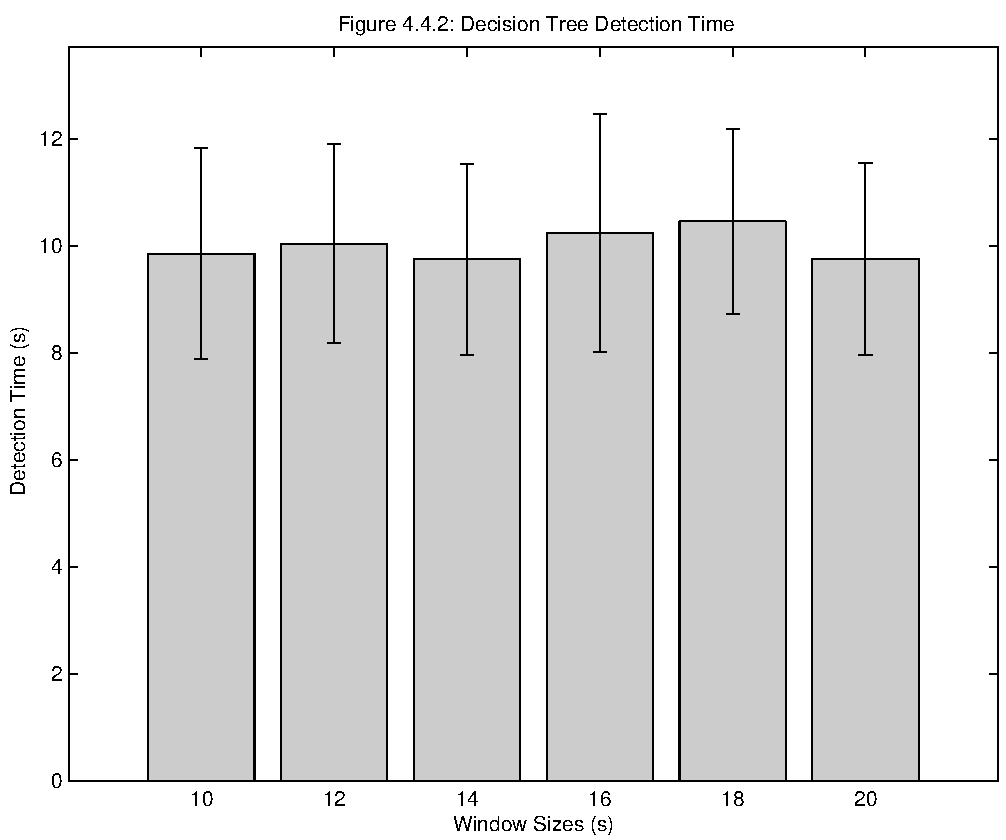
\includegraphics[scale=0.4]{osu_hmm_dt_det.pdf}
 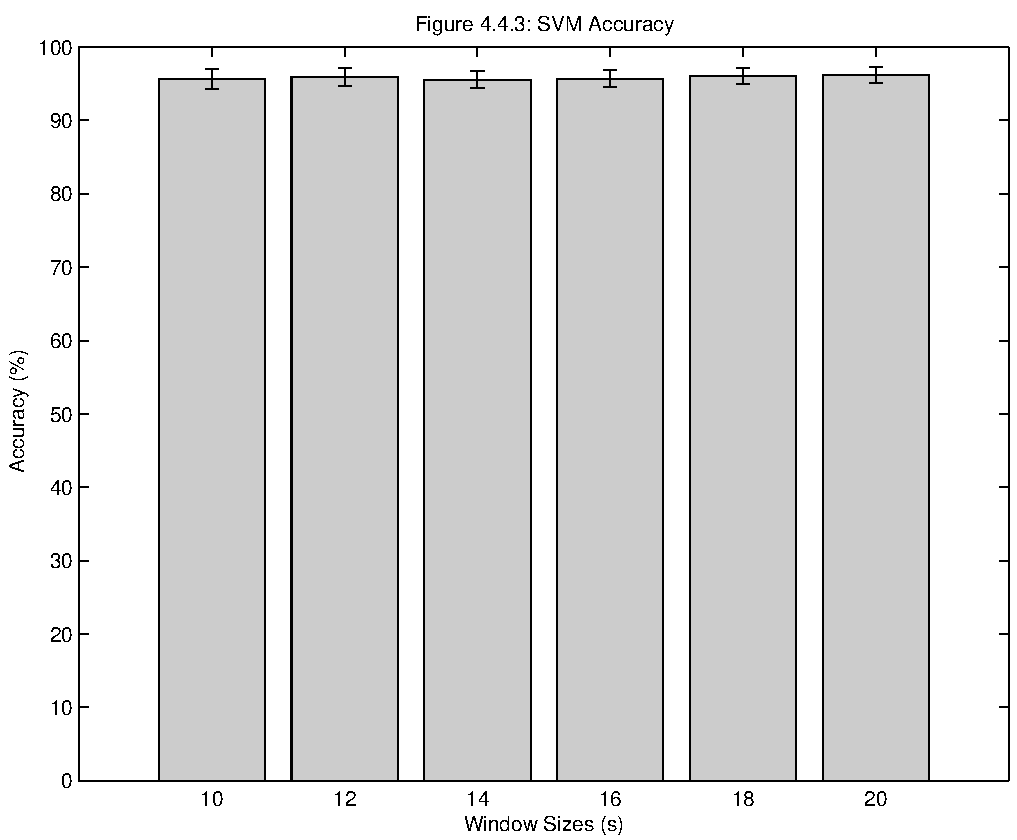
\includegraphics[scale=0.4]{osu_hmm_svm_acc.pdf} \hspace{1em}\vspace{1em}
 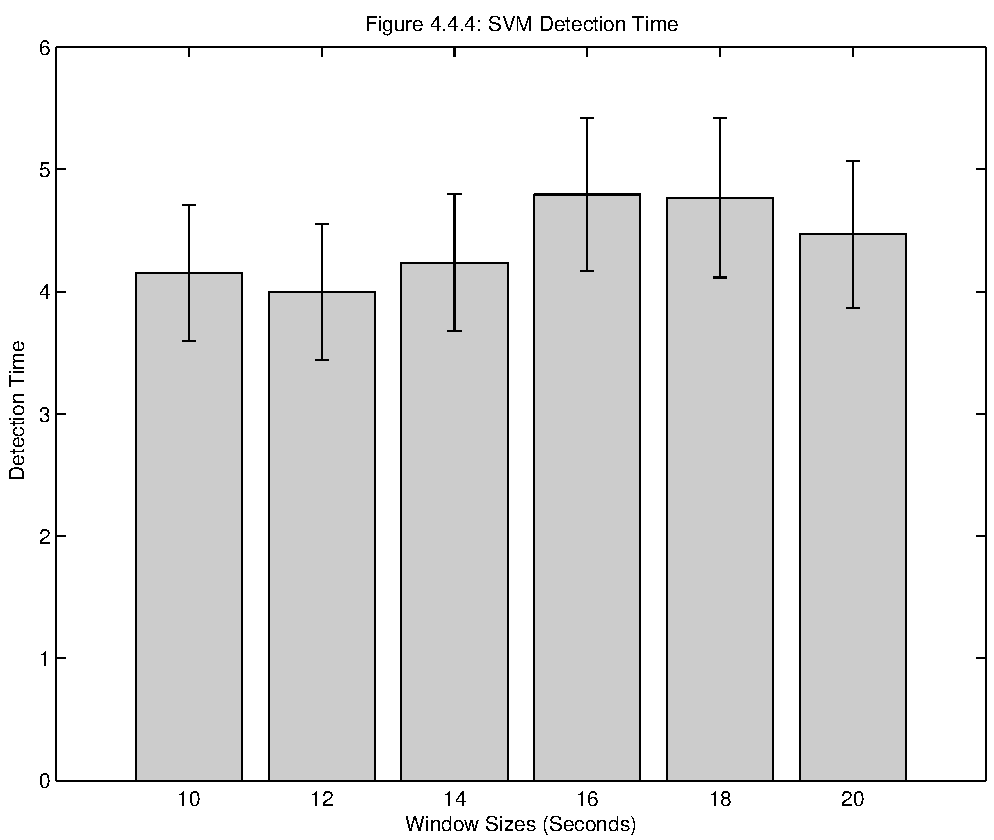
\includegraphics[scale=0.4]{osu_hmm_svm_det.pdf}
 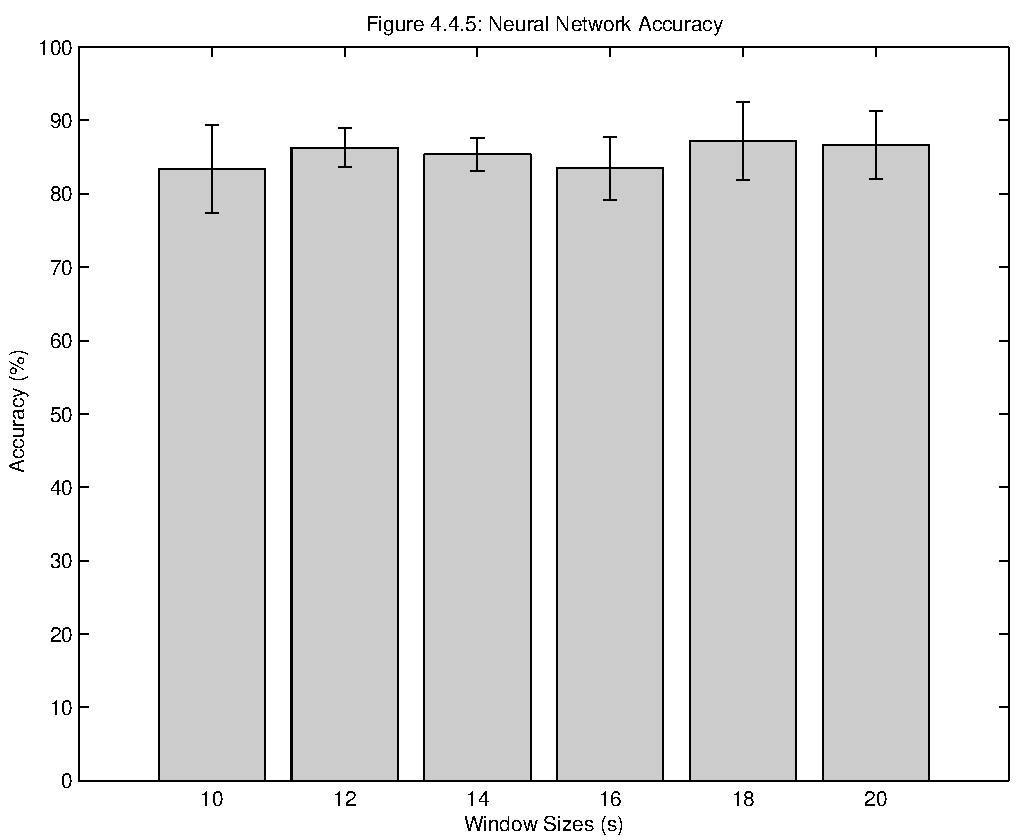
\includegraphics[scale=0.4]{osu_hmm_nnet_acc.pdf} \hspace{1em}
 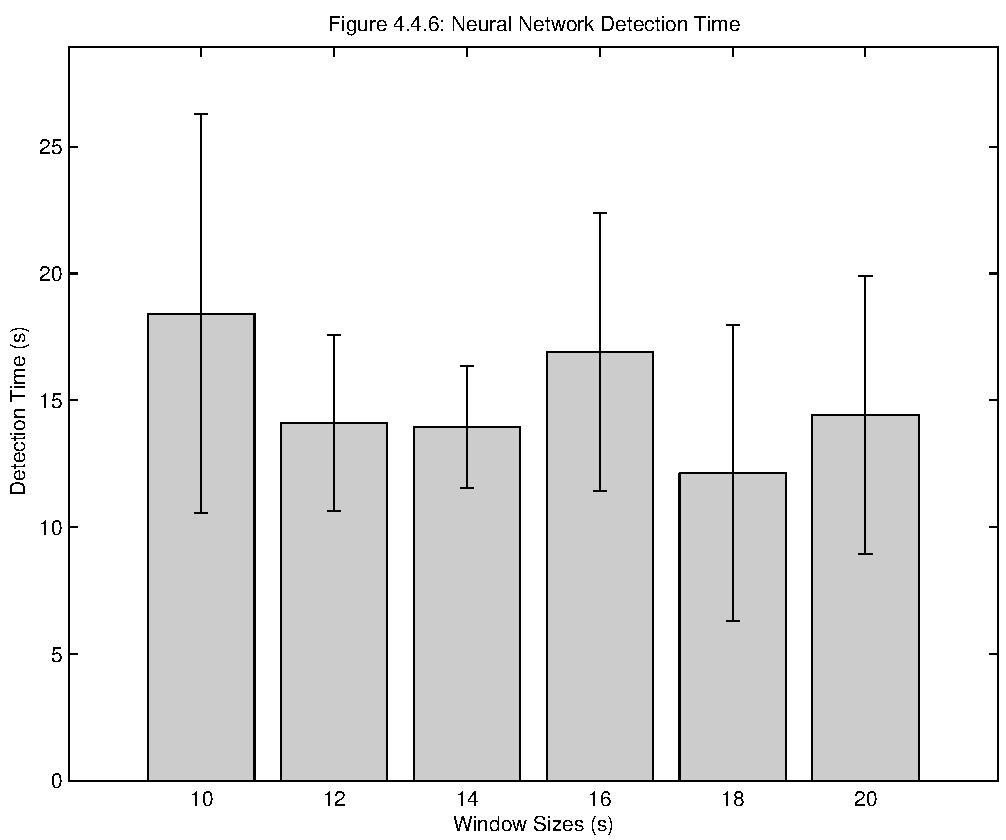
\includegraphics[scale=0.4]{osu_hmm_nnet_det.pdf}
 \caption{OSU Hip HMM Results.
  Graphs are organized into rows by base classifier, and columns by evaluation
  metric. HMM results were averaged over 10 splits into training
  (base classifier), validation, training (HMM), and testing datasets, along with bars
  showing one standard error.}
 \label{fig:osu_hmm}
\end{figure}

\begin{figure}[H]
 \centering
 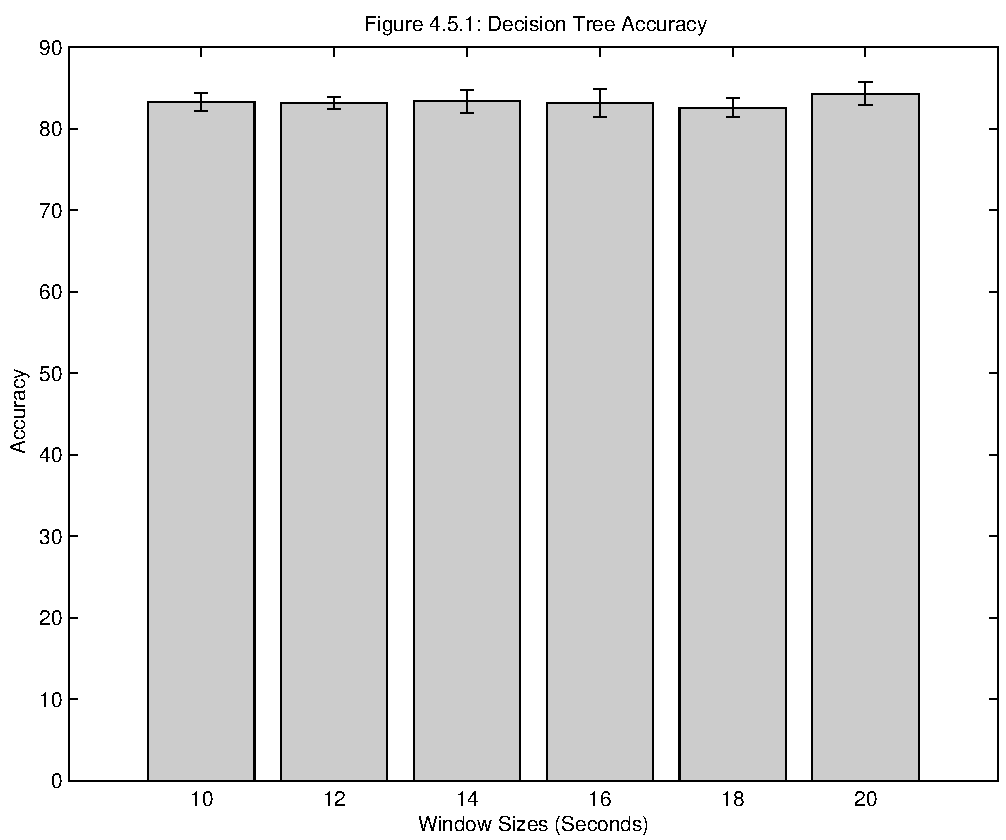
\includegraphics[scale=0.4]{lime1_hmm_dt_acc.pdf} \hspace{1em}\vspace{1em}
 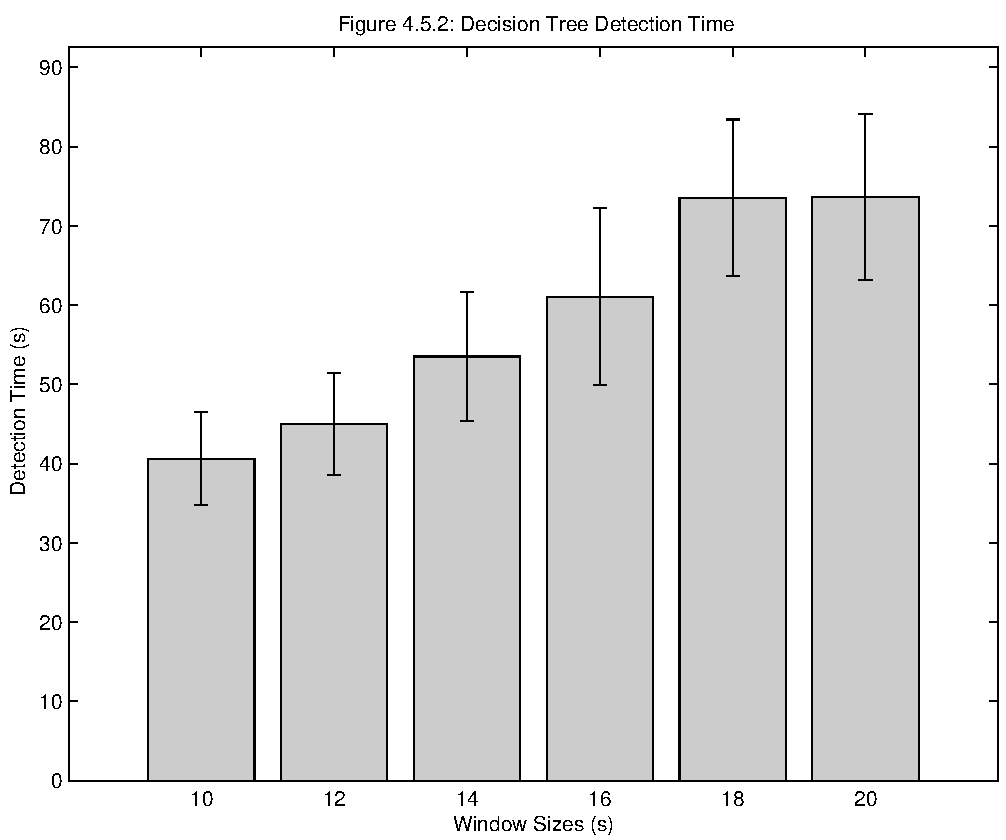
\includegraphics[scale=0.4]{lime1_hmm_dt_det.pdf} 
 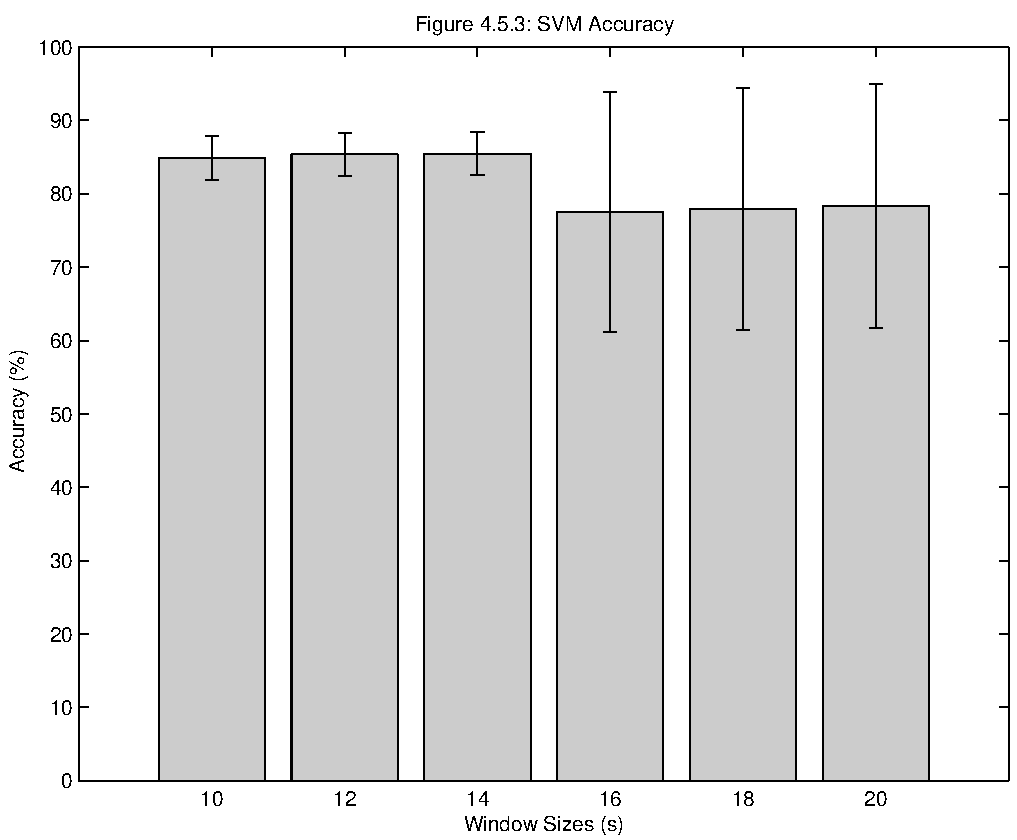
\includegraphics[scale=0.4]{lime1_hmm_svm_acc.pdf} \hspace{1em}\vspace{1em}
 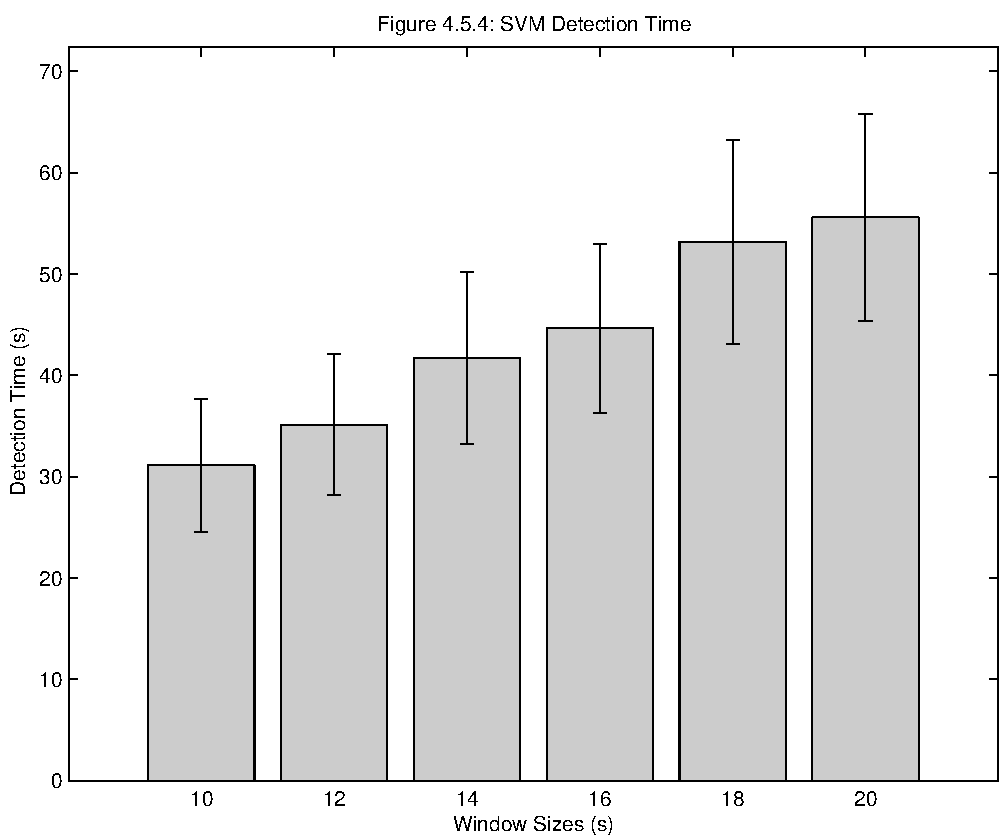
\includegraphics[scale=0.4]{lime1_hmm_svm_det.pdf} 
 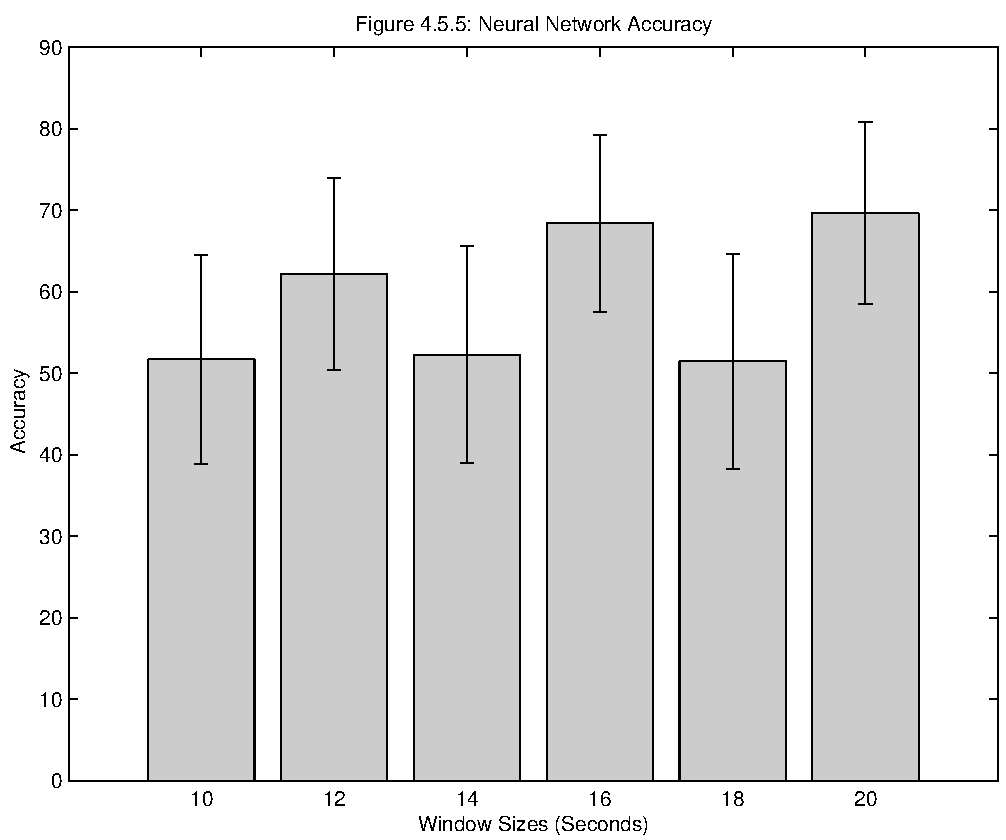
\includegraphics[scale=0.4]{lime1_hmm_nnet_acc.pdf} \hspace{1em}
 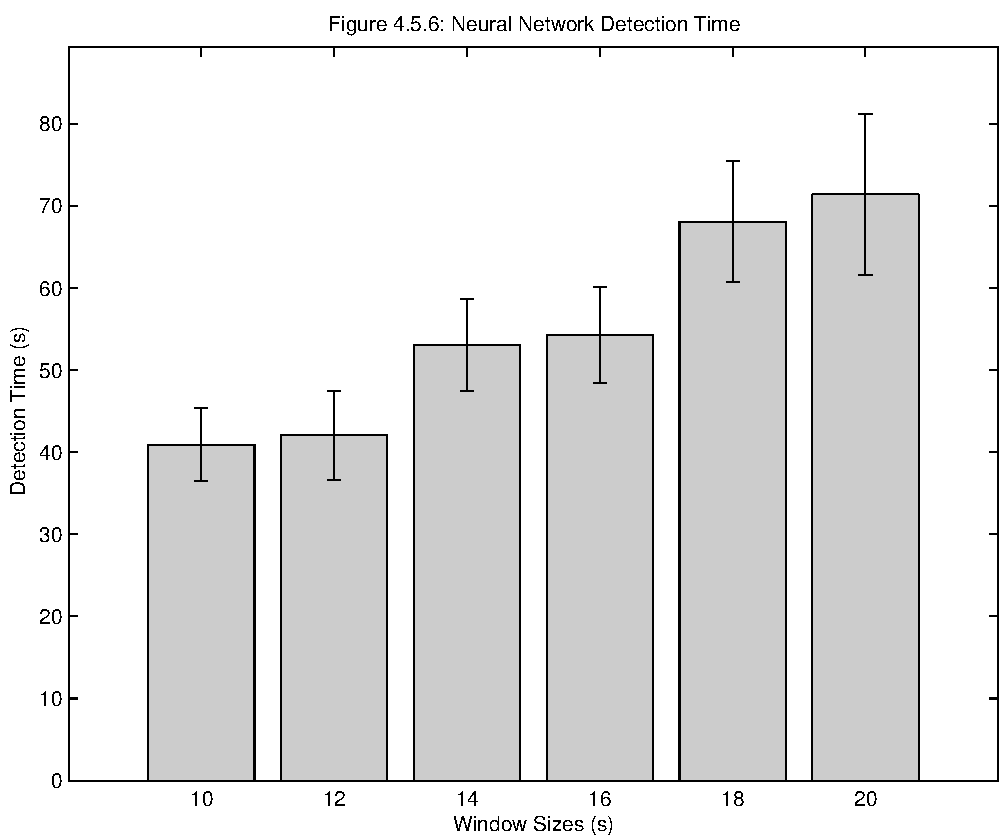
\includegraphics[scale=0.4]{lime1_hmm_nnet_det.pdf} 
 \caption{LiME Day 1 HMM Results}
 \label{fig:lime1_hmm}
\end{figure}

\begin{figure}[H]
 \centering
 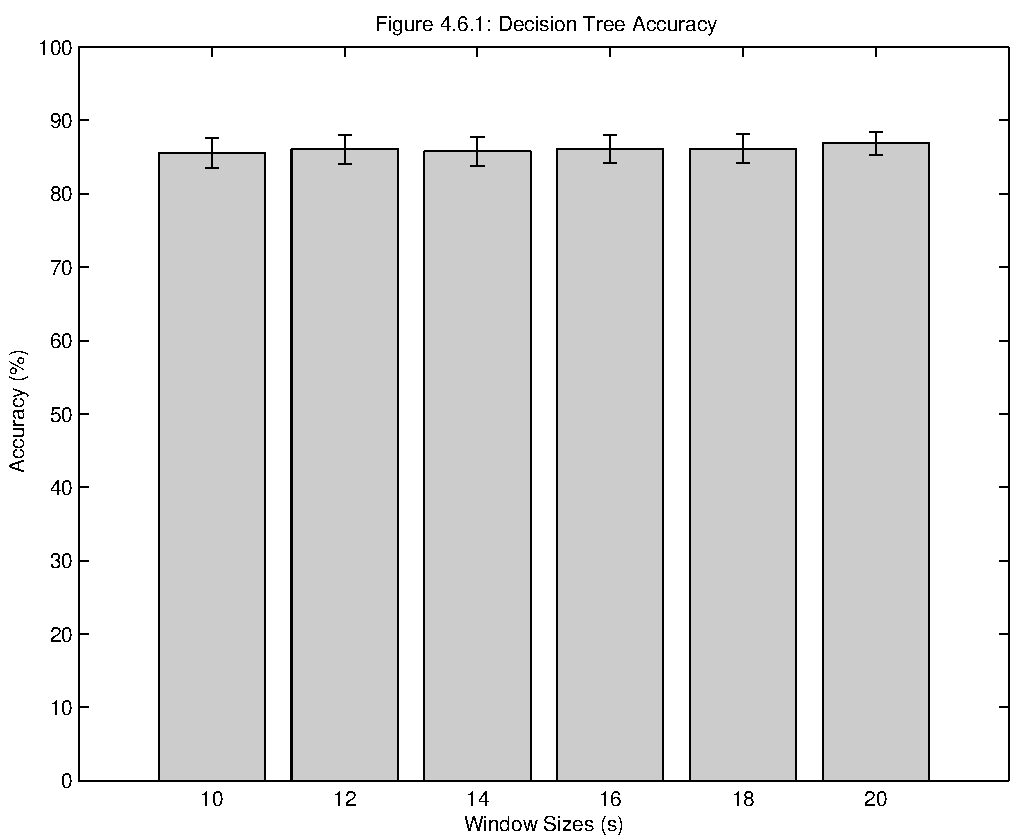
\includegraphics[scale=0.4]{lime2_hmm_dt_acc.pdf} \hspace{1em}\vspace{1em}
 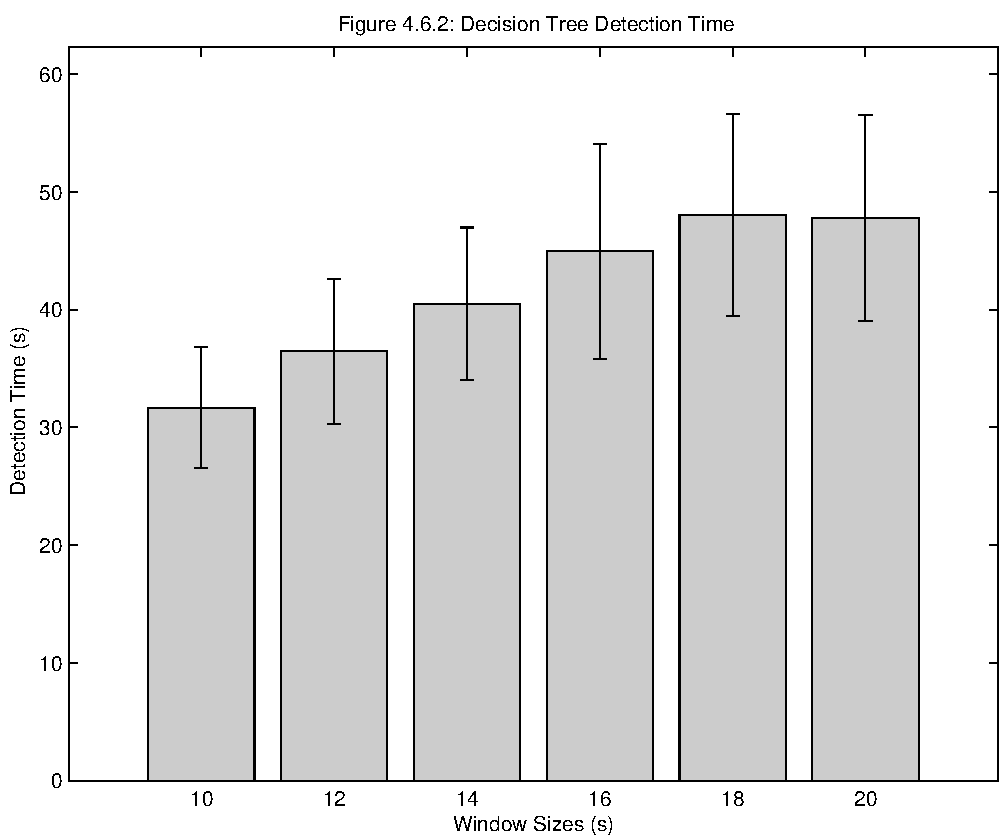
\includegraphics[scale=0.4]{lime2_hmm_dt_det.pdf}
 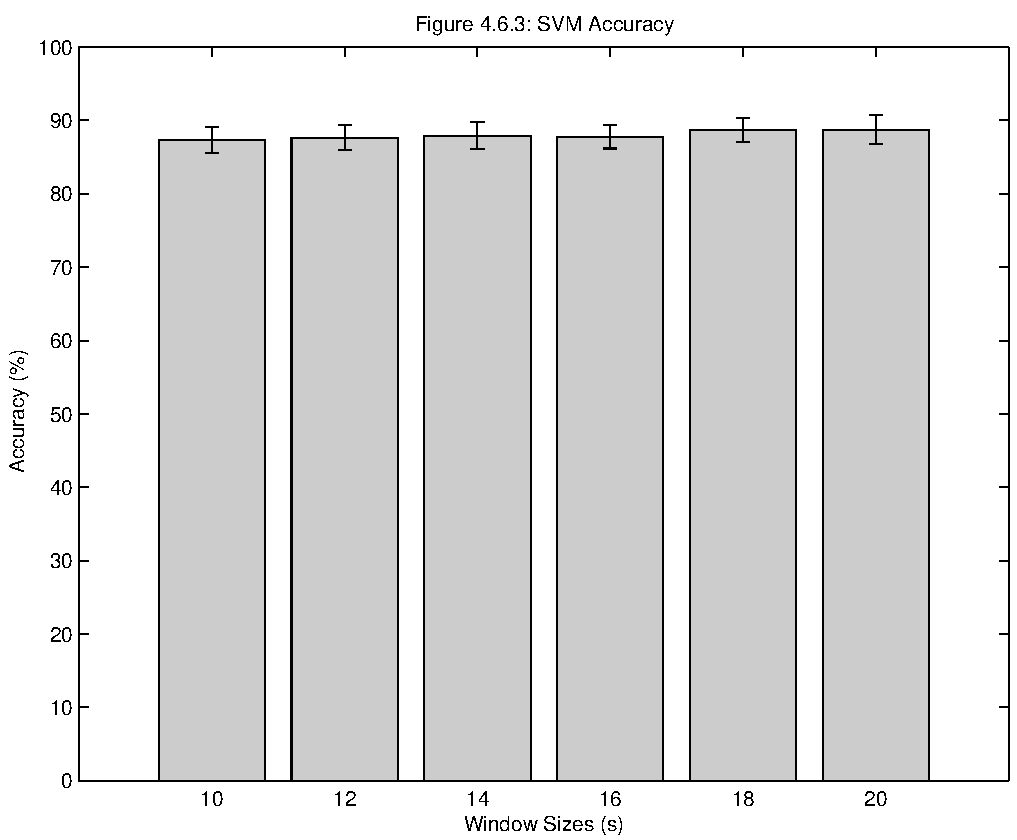
\includegraphics[scale=0.4]{lime2_hmm_svm_acc.pdf} \hspace{1em}\vspace{1em}
 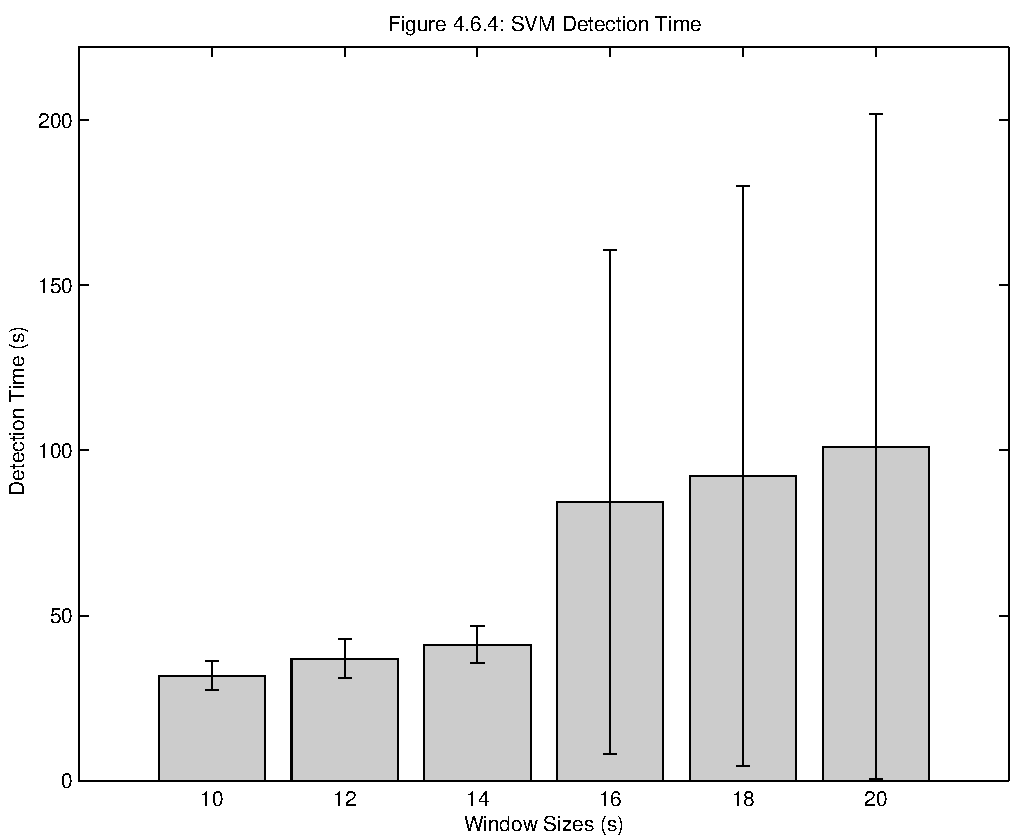
\includegraphics[scale=0.4]{lime2_hmm_svm_det.pdf}
 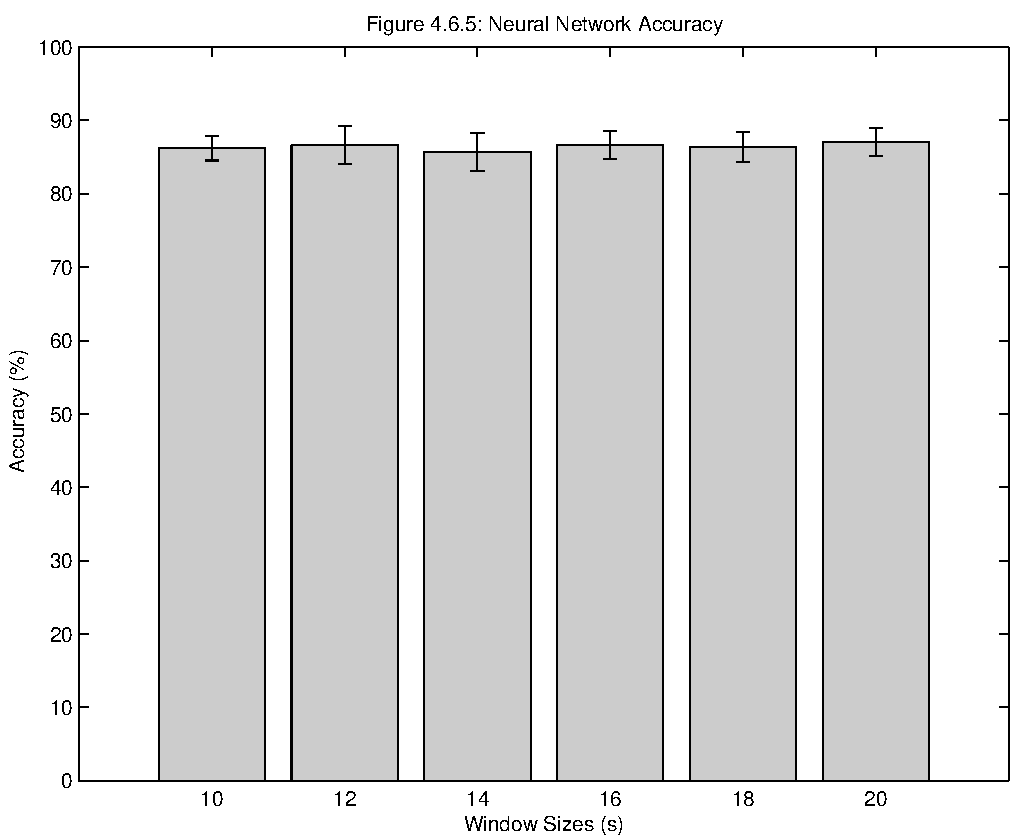
\includegraphics[scale=0.4]{lime2_hmm_nnet_acc.pdf} \hspace{1em}
 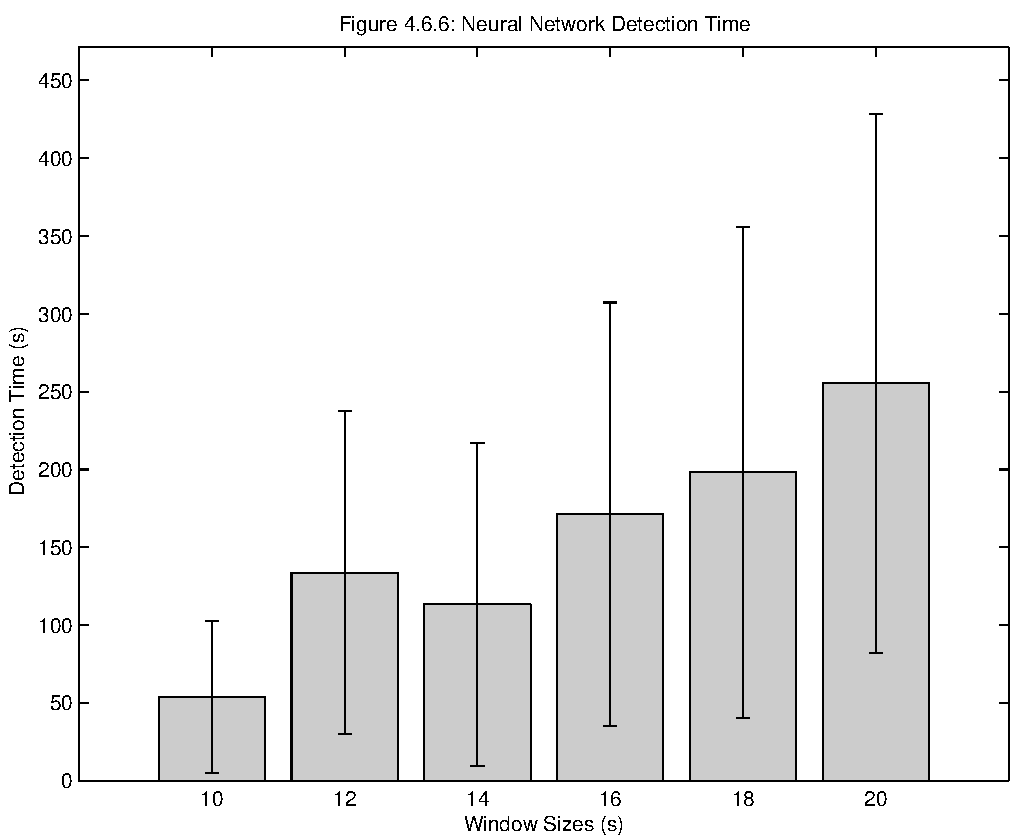
\includegraphics[scale=0.4]{lime2_hmm_nnet_det.pdf}
 \caption{LiME Day 2 HMM Results}
 \label{fig:lime2_hmm}
\end{figure}

\newpage

\section{Discussion}

Our results clearly show that the HMM approach outperformed the change-point
detection approach, both in terms of accuracy and detection time, regardless of
the dataset and base classifier. This was expected, as our change-point
detection algorithms did not perform expecially well at predicting changes at
the correct locations, and also because HMMs are a well-established and well-
grounded approach in sequential, time-oriented domains.

A further point of interest was that SVM clearly beat out the other two
base classifiers, and that the faster and simpler decision tree model did fairly
well against neural networks. This result is significant because much of the
previous research that has formulated activity detection as a supervised learning
problem has used neural networks exclusively.
